\documentclass[UKenglish]{lipics-v2019}

\usepackage[dvipsnames]{xcolor}

\usepackage[utf8]{inputenc}
\usepackage{graphicx}
\usepackage{amssymb}
\usepackage{amsfonts}
\usepackage{amsthm}
\usepackage{wrapfig}
\usepackage{makecell}
\usepackage{xspace}
\usepackage{multirow}
\usepackage{comment}
\modulolinenumbers[5]

\graphicspath{{./figures/}}

\newcommand{\myremark}[4]{\textcolor{blue}{\textsc{#1 #2:}} \textcolor{#4}{\textsf{#3}}}
\newcommand{\frank}[2][says]{\myremark{Frank}{#1}{#2}{SeaGreen}}
\newcommand{\patrick}[2][says]{\myremark{Patrick}{#1}{#2}{Plum}}
\newcommand{\maarten}[2][says]{\myremark{Maarten}{#1}{#2}{Red}}
\newcommand{\ivor}[2][says]{\myremark{Ivor}{#1}{#2}{Blue}}

\usepackage{tabularx,booktabs}

\newtheorem{condition}{Condition}
\newtheorem{conjecture}{Conjecture}
\newtheorem{observation}{Observation}

\newcommand{\etal}{\textnormal{et al.}\xspace}

% macro for making mathcal definitions
\newcommand{\mkmcal}[1]{\ensuremath{\mathcal{#1}}\xspace}

% common mathcal definitions
\newcommand{\G}{\mkmcal{G}}
\newcommand{\Lst}{\mkmcal{L}}
\newcommand{\T}{\mkmcal{T}}
\newcommand{\C}{\mkmcal{C}}
\newcommand{\X}{\mkmcal{X}}
\newcommand{\D}{\mkmcal{D}}
\newcommand{\M}{\mkmcal{M}}
\newcommand{\E}{\mkmcal{E}}
\newcommand{\BB}{\mkmcal{B}}
\renewcommand{\S}{\mkmcal{S}}
\renewcommand{\H}{\mkmcal{H}}

\newcommand{\geod}{\pi\xspace}

% macro for mathbb definitons, for definiton of the naturals N, and booleans
\newcommand{\mkmbb}[1]{\ensuremath{\mathbb{#1}}\xspace}

\newcommand{\R}{\mkmbb{R}}

\def\polylog{\operatorname{polylog}}

\title{Trajectory Visibility}
\titlerunning{Trajectory Visibility}


\author{Patrick Eades}{University of Sydney}{patrick.eades@sydney.edu.au}{}{}
\author{Ivor van der Hoog}{Utrecht University}{i.d.vanderhoog@uu.nl}{}{}
\author{Maarten Löffler}{Utrecht University}{m.loffler@uu.nl}{}{}
\author{Frank Staals}{Utrecht University}{f.staals@uu.nl}{}{}
\authorrunning{P. Eades, I. van der Hoog, M. L\"offler, and F. Staals}
\Copyright{Patrick Eades, Ivor van der Hoog, Maarten L\"offler, and Frank Staals}%mandatory, please use full first names. LIPIcs license is "CC-BY";  http://creativecommons.org/licenses/by/3.0/

\begin{document}

\maketitle

\begin{abstract}
  \frank{we should write an abstract}
\end{abstract}





\newpage


\section {Introduction}

We consider the following question. Two entities are following different trajectories in an environment with obstacles which block visibility. Can they, at any time, see each other? 

\subparagraph {Trajectories.}

A recent dramatic increase in the availability of low-cost, internet connected GPS tracking devices has driven considerable interest in spatio-temporal data (commonly called {\em trajectories}) across fields including GIScience, databases, and computational geometry. 
Problems studied recently in computational geometry include detecting and describing flocks \cite{AnderssonGLW07, BenkertGHW08, LaubeKI04} and hotspots, clustering and categorising trajectories, map construction and others~\cite{bbgll-dcpcs-11,grsc-pcecu-07,gs-tcmrm-99,lhw-tc-07,vgk-dsmt-02}.
Formally, a trajectory is a 
sequence of time-stamped locations 
in the plane, or more generally in $\R^d$, which
models the movement of an entity.
Trajectory data is obtained by tracking the movements of e.g. animals \cite{BovetB88,Calenge200934,gal-nmibc-09}, hurricanes \cite{Stohl1998947}, traffic \cite{lltx-dftf-10}, or other moving entities \cite{dwf-rpm-09} (pedestrian crowds, sportspeople, political sentiment, stock prices,\ldots) over time.
It is beyond the scope of this paper to review the extensive literature on trajectory analysis; we refer the reader to the excellent survey by Gudmundsson~\etal~\cite{GudmundssonLW17}.

\subparagraph {Visibility.}
Two objects, amidst a number of obstacles, are \emph{visible} from each other if the segment between them is not obstructed. 
Visibility is one of the most studied topics in computational geometry~\cite {moet,welzl1985constructing,POCCHIOLA1996279}. 
Even more so in adjacent fields such as computer graphics~\cite {Durand00amultidisciplinary}, Geographic Information Science (GIS)~\cite{FM03}, and robotics~\cite {moet}, to name just a few.
Within computational geometry, Gosh and Giswani compiled a survey of {\em unsolved} problems in this area~\cite {Ghosh:2013:UPV:2543581.2543589}.
Core visibility problems in computational geometry include {\em ray shooting}~\cite{10,13,17,20}, guarding~\cite {Chvatal75,Fisk78,survey}.
For more information about visibility problems, refer to O'Rourke's book \cite{ORourke87} ch. 28, and the surveys by Durant \cite{durand2000multidisciplinary} and Gosh~\cite{Ghosh:2013:UPV:2543581.2543589}. 

\subparagraph {Trajectory visibility.}


\begin{figure} [tb]
	\centering 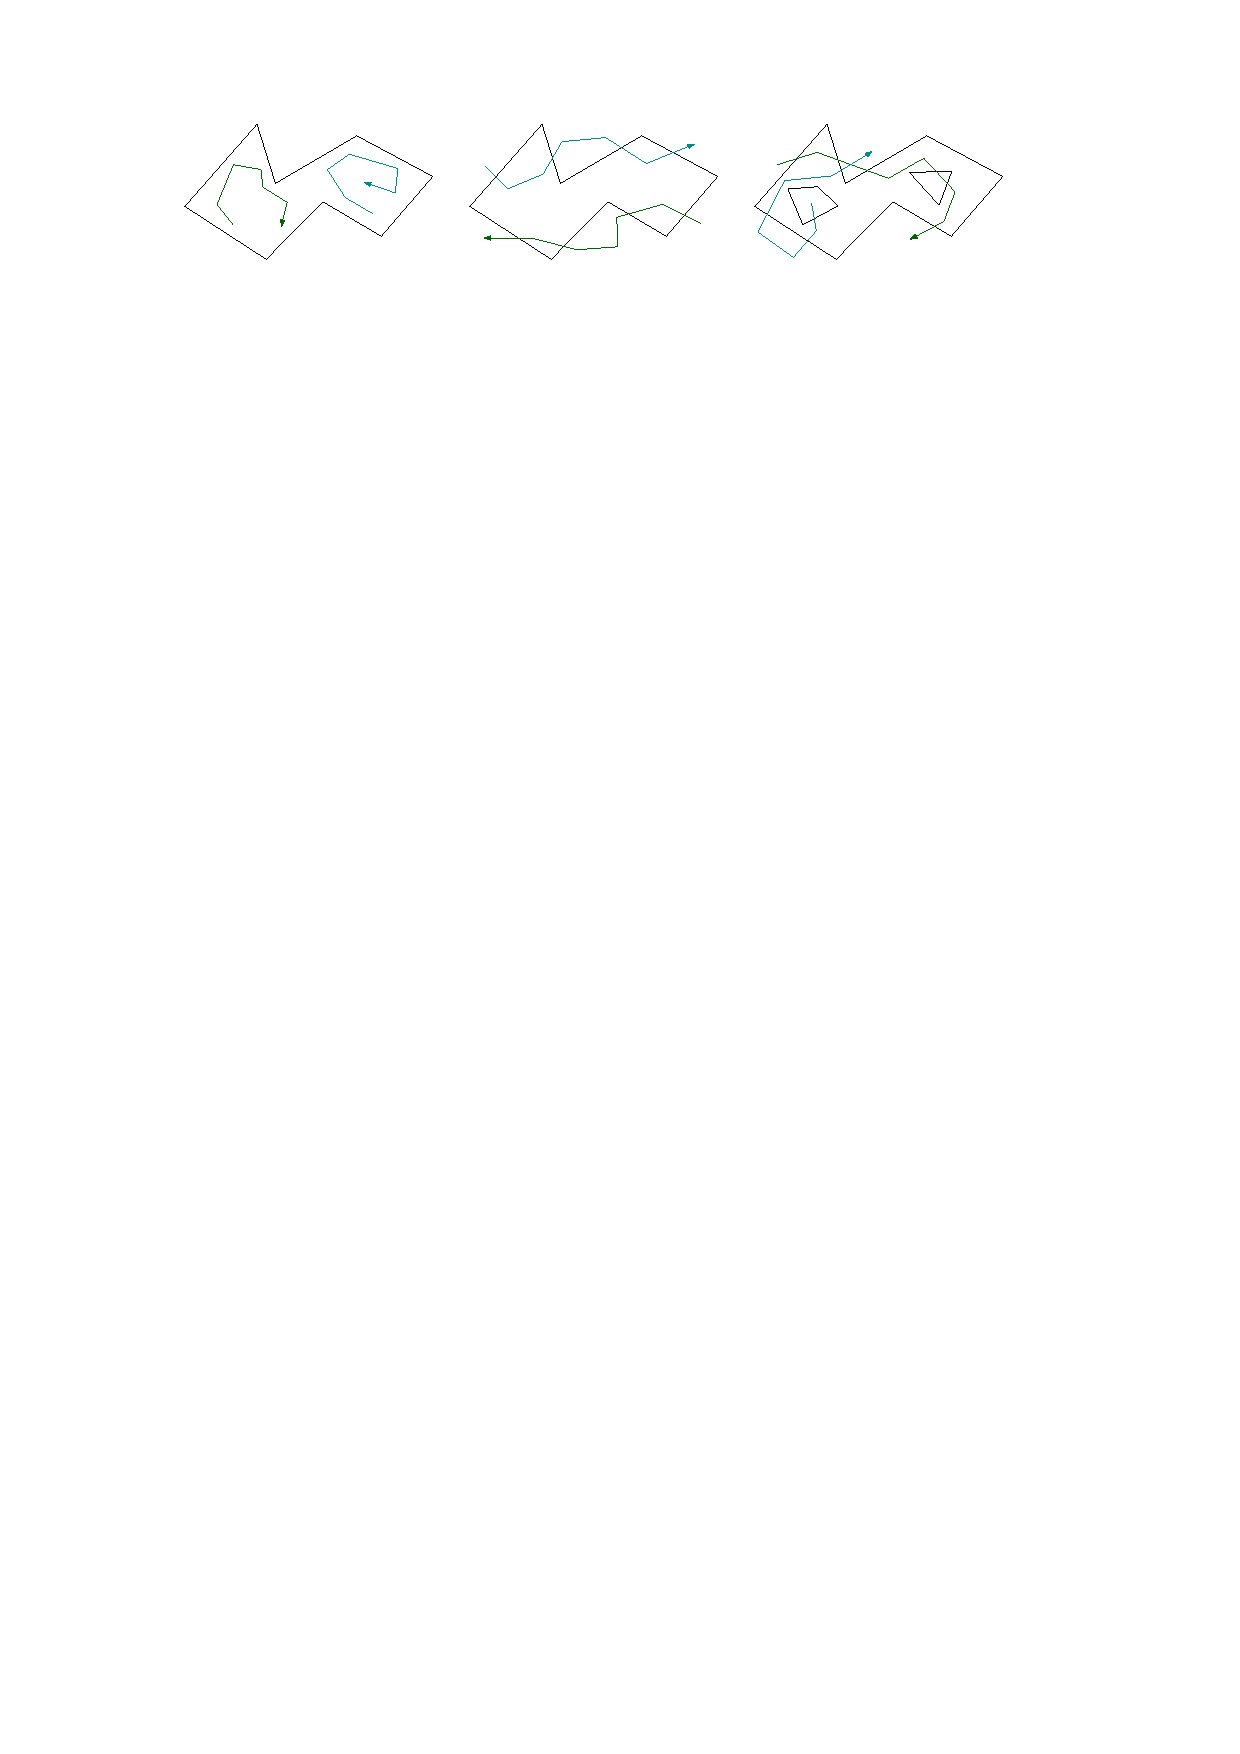
\includegraphics {variants} 
	\caption
	{
	  Different versions of the question:
	  two trajectories inside a simple polygon (left);
	  two trajectories intersecting a simple polygon (middle);
	  or two trajectories in a polygonal domain (right).
	}  
	\addtolength{\belowcaptionskip}{-50pt}
	\label{fig:variants}
\end{figure}

Somewhat surprisingly, given the amount of research on both trajectories and visibility, not much previous work exists on their combination.
%
In this paper, we study the following fundamental question.
  Given a simple polygon or polygonal domain $P$ with $n$ vertices and given two entities $q$ and $r$ that both traverse a trajectory of $\tau$ vertices each, is there a time $t$ at which two entities see each other?
  We assume that $q$ and $r$ move with constant (but possibly different) speeds between trajectory vertices, and cannot see though the edges of $P$.
  We distinguish several variants depending on whether $P$ is a simple polygon or a polygon with holes, and whether the trajectories are allowed to intersect $P$ (i.e. vehicles moving through fog, animals moving though foliage) or not (e.g. pedestrians moving among buildings, ships moving on water bodies). Refer to Figure~\ref {fig:variants}.
%
%Part of the reason may be that studying trajectories in {\em context} is still relatively new area, and context is essential for meaningful question.
%On the other hand, the role of {\em time} is essential in this scenario: we are not interested whether there exists visibility between two geometric shapes, but rather whether there exists a {\em time} at which two point objects are visible. This makes the question fundamentally different from existing work in visibility.

Note that we are only interested in the question whether there {\em
  exists} a time at which the two entities see each other. % (more complex questions may be considered, we start with the most basic version; refer also to Section~\ref {sec:conclusions}).
This implies we can decompose the problem: the answer is {\em no} if and only if the answer is no between all two consecutive time stamps.
When considering this question, two fundamentally different approaches come to mind. On the one hand, when $\tau$ is small compared to $n$, the best approach may be to simply solve the problem for each time interval separately. On the other hand, when $\tau$ is large compared to $n$, it may be more efficient to spend some time on preprocessing $P$ first, if this allows us to spend less time per time interval.
We therefore distinguish between the {\em algorithmic} and the {\em data structure} question.

\subparagraph {Data structures for visibility.}

Data structures for point-to-point visibility are well-known. 
Chazelle \etal~\cite{chazelle1994ray} present a linear-size data structure on a simple polygon $P$ which for any ray originating from a point, can determine the first edge hit by the ray in logarithmic time. Entity $r$ is visible from $q$ if and only if the ray from $q$ to $r$ does not hit an edge before reaching $r$. Guibas and Hersberger \cite{GUIBAS1989126} present a linear-size data structure on a simple polgyon which can return the shortest path between a pair of query points in logarithmic time. Note that $q$ and $r$ are mutually visible if and only if their shortest path is a single line segment.
Guibas and Hershberger's work concludes a series of triangulation-based shortest path algorithms for a simple polygon including Lee and Preparata \cite{LeeP84}, Reif and Storer \cite{ReifS85} and Guibas~\etal~\cite{GuibasHLST87}.
Lee and Preparata \cite{LeeP84} find the shortest path (and with it the visibility) between two points in a simple polygon in linear time, if linear time triangulation is used.
%which implicitly solves visibility between two points.


Visibility of a moving object is an old subject within visibility that recently has gained attention within the computational geometry community. Bern \etal~\cite{bern1994visibility} and  Mulmuley \cite{mulmuley1991hidden} study maintaining the visibility polygon of a point that moves over a straight path. 
Aronov \etal~\cite{aronov2002visibility} demonstrate a kinetic algorithm that tracks the visibility polygon of a moving query point $q$. The most recent result on visibility and motion is by Diez \etal~\cite{DKRRS2017KineticAPSPEuroCG} who show how to maintain the shortest path between two moving entities using a kinetic data structure. The entities can see one another if and only if their shortest path is a line segment and thus this kinetic data structure can be used to compute visibility between two moving entities. 
A large body of work also exists on the complementary problem of planning trajectories under visibility constraints~\cite {6907405}.


\newcolumntype{Y}{>{\centering\arraybackslash}X}
\begin{table}[t]
    \centering
    \begin{tabularx}{\linewidth}{ccYYYYYY}
      \toprule
      $q$ & $r$ & $P$ & algorithm & \multicolumn{3}{c}{data structure} & source \\
          &     &     &           & space & preprocessing & query & \\
        \midrule
        %
        $\bullet$ & $\bullet$ & S or I &  $\Theta(n)$ & $\Theta(n)$ & $\Theta(n)$ & $\Theta(\log n)$ & \cite{guibas1989optimal} \\
                  &           & D      & $\Theta(n)$ & $\mathcal{O}()$ & $\mathcal{O}()$ & $\mathcal{O}()$ & \cite{POCCHIOLA1996279}
        \\[0.6em]
        %
        $\bullet$ & $\slash$ & S & $\Theta(n)$ & $\Theta(n)$ & $\mathcal{O}(n \log n)$ & $\Theta(\log n)$ & Section~\ref{sec:pointline} \\
                  &          & I & $\Theta(n)$ & $\mathcal{O}(n^{2} \log n)$ & $\mathcal{O}(n^{2 })$ & $\mathcal{O}(n^{\frac{7}{8} })$ & Section~\ref{sec:pointline} \\
                  &          & D & $\mathcal{O}(n \log n)$ & $\mathcal{O}(n^4 \log n)$ & $\mathcal{O}(n^{4  })$ & $\mathcal{O}(n^{7/8 })$ &  Section~\ref{sec:pointline}
        %
        \\[0.6em]
        $\slash$ & $\slash$ & S & $\Theta(n)$ & $\mathcal{O}(n \log n)$ & $\mathcal{O}(n^{1 })$ & $\mathcal{O}(n^{3/4 })$ & Section~\ref{sec:lineline} \\
                 &          & I & $\Theta(n)$ & $\mathcal{O}(n^{c})$ & $\mathcal{O}(n^{c+\varepsilon})$ & $\mathcal{O}(\log^c n)$ & Section~\ref{sec:lineline}  \\
                 &          & D & $\mathcal{O}(n \log n)$ & $\mathcal{O}(n^c)$ & $\mathcal{O}(n^{c })$ & $\mathcal{O}(\log^c n)$ & Section~\ref{sec:lineline} \\
        \bottomrule
    \end{tabularx}
        \caption{Results using partition trees. The two left-most
          columns specify if the query entity is a point ($\bullet$)
          or line segment ($\slash$). The third column specifies if
          the domain $P$ is a simple polygon (S), a polygon where the
          query segments may intersect $P$ (I) or a polygonal domain
          with $n$ vertices (D). \frank{Check these results; I'm not
            sure I believe the $O(n)$ bounds for the algorithmic problems}}
    \label{tab:results}
    % \vspace{-20pt}
\end{table}

\subparagraph {Our Results.}
  Our results for when the two trajectories are single line segments are summarized in Table~\ref {tab:results}; we additionally consider the case where both are points (the entities are stationary) for comparison, and the case where {\em one} entity is a point and the other is a segment as an easier version of the problem leading up to our more general results.
 %
  In Section~\ref{sec:alg}, we discuss our algorithmic results.
  If we are allowed to preprocess $P$ we use multi-level data structures. As the base level of thesestructures we either use the shortest path structure from Guibas and Hershberger \cite{guibas1989optimal} or the visibility polygon retrieval structure from Aronov \etal~\cite{aronov2002visibility}. At the top level we transform the visibility query into an intersection query between an algebraic query object and a pre-stored geometric object from the lower levels. There we encounter a sub-problem of independent interest: can we preprocess a convex polygon $P'$ such that we can answer intersection queries with degree-2 curve segments in sublinear time; 
  
  In Section~\ref{sec:intersectionsearch} we present the solution to this sub-problem. The techniques presented in that section are a good example of the techniques used throughout this paper. Section~\ref{sec:pointline} contains the data structure result for when one entity is stationary and the general case is presented in Setion~\ref{sec:lineline}.
\frank{why is there a $\varepsilon$ in our table for the second to
  last row?}

  
\section{Preliminaries}
\label{sec:prelims}

\subsection{Linearization}
\label{subsec:}

\frank{Actually, this is more about linearization then about
  semi-alg. range searching no?. I.e. We don't care about range
  searching, but about intersection searching!}

\subparagraph{Semi-algebraic range searching.}
Let $X$ be a set of $n$ geometric objects in $\mathbb{R}^d$, where each object is parametrized by a vector $\vec{x}$ (e.g. a point is parametrized by a vector of its coordinates). Let $\Gamma$ be a family of geometric regions (called semi-algebraic ranges) in $\mathbb{R}^d$ where each region $G \in \Gamma$ is bound by an algebraic curve $\gamma$ which is parametrized by a vector $\vec{a}$. Agarwal \etal~\cite{agarwal2013range} are interested in preprocessing $X$, such that for any range $G \in \Gamma$, we can report which objects of $X$ intersect $G$. They show the following: suppose you can derive a predicate function $F(\vec{x}, \vec{a})$ which for any pair $(x,G)$ patametrized by $(\vec{x}$, $\vec{a})$ outputs a real number, such that $F(\vec{x}, \vec{a}) \le 0$ if and only if $x$ and $G$ intersect. Suppose you can rewrite the function into the form  $F(\vec{x}, \vec{a}) =  g_0(\vec{a}) + \sum_{i=1}^k g_i(\vec{a})f_i(\vec{x})$ where $f_i$ and $g_i$ are polynomials dependent only on $\vec{x}$ and $\vec{a}$ respectively (we call this \emph{linearization}). Then Agarwal \etal show how to transform this $d$-dimensional semi-algebraic range searching problem into a halfspace range searching problem into $\mathbb{R}^k$. Specifically, Agarwal \etal prove that you can map any $d$-dimensional point $\vec{x}$ to the $k$-dimensional point $f(\vec{x}) = (f_1(\vec{x}), f_2(\vec{x}), \dots f_k(\vec{x}))$, and any query range to the $k$-dimensional halfspace $G(\vec{a}) = \left\{ \vec{y} \in \mathbb{R}^k \mid g_0(\vec{a})  + \sum_i^k g_i(\vec{a})y_i  \le C \right\}$ and that $\vec{x}$ intersects $G$ if and only if $f(\vec{x})$ is contained in $G(\vec{a})$. Refer to Appendix~\ref{appx:rangesearch} for more information about semi-algebraic range searching.




\subparagraph{Halfspace range queries.}
Semi-algebraic range searching transforms an intersection query into a $k$-dimensional halfspace range query. $k$-dimensional halfspace range searching can be solved using partition trees \cite{chan2012optimal} which use $\Theta(n)$ space, $\mathcal{O}(n \log n)$ preprocessing time and has an expected query time of $\mathcal{O}(n^{1 - \frac{1}{k}})$ (worst-case bounds exists with an additional polylog factor). Halfspace emptyness queries (which are used to determine \emph{if} there is an intersection) have $\mathcal{O}(n^{1 - \frac{2}{k+1}})$ query time. Alternatively one can use cutting trees \cite{chazelle1993cutting} which use $\mathcal{O}(n^k)$ space and preprocessing time but achieve $\mathcal{O}(\log^k n)$ query time.
%




\subparagraph{Intersecting line segments with a quadratic curve segment.}
Applying semi-algebraic range searching works in two steps: first you algebraically describe what query you are interested in (in this case an intersection between $\gamma$ and an edge $e \in E$), then you linearize this expression into $k$ terms as described in Section~\ref{sec:prelims}. This transforms the algebraic query into a $k$-dimensional halfspace range emptyness. It might be tempting to immediately implore this technique to solve our intersection query. However the more complicated the algebraic expression, the higher the number $k$ will be. In Appendix~\ref{appx:rangesearch} we prove the following lemma which leads to a result which might be sub-linear, but not very practical:

\begin{lemma}
\label{lemma:15000}
We can preprocess a set $E$ of \emph{arbitrary} line segments using $\mathcal{O}(S(15000))$ space and $\mathcal{O}(C(15000))$ construction time, such that an intersection (if any exists) between an arbitrary degree-2 curve segment $\gamma$ and an edge in $E$ can be found in $\mathcal{O}(Q(15000))$ time.
\end{lemma}


\subsection{An algorithm for testing visibility}
\label{subsec:oneshots}

We will begin by briefly considering visibility between two trajectories when the obstacles are not known beforehand. We consider two versions of this problem: where the obstacles consist of $n$ arbitrary line segments, and a restriction where the line segments form the boundary of a simple polygon. We show these problems can be solved in $\mathcal{O}(n \log n)$ and $\mathcal{O}(n)$ time respectively.

Consider the times at which a single line segment blocks visibility between $q$ and $r$, these times consist of up to two sub-intervals of $[0, 1]$, which can be computed in constant time. Thus $n$ line segments induce a set of $\mathcal{O}(n)$ obstructed time intervals, which can be computed in $\mathcal{O}(n)$ time. Their union can be computed in $\mathcal{O}(n \log n)$ by sorting. If this union is equal to $[0, 1]$ then at every time there is a line segment which prevents $q$ and $r$ seeing each other, if not then any uncovered time is a moment at which the segment between $q$ and $r$ is not obstructed by any line segment and hence $q$ and $r$ can see each other.

\patrick{it seems quite reasonable that if the edges are already sorted we can do this in O(n) but this is a bit evasive to prove}

\patrick{There is not quite a lower bound from the measure problem, there is almost one}

\frank{Say something about the lowerbound; plan was to go via
  (batched) predecessor queries in the comparison model}


\section{Intersecting a curve segment and a convex polygon}
\label{sec:intersectionsearch}
Suppose we are given a set $E$ of $n$ edges which form a convex polygon $P_E$. We want to preprocess $E$, such that given any segment $\gamma$ of an arbitrary degree-2 polynomial curve in the plane, we can test whether $\gamma$ intersects $P_E$ in sub-linear time. This check can be performed easily in linear time by testing for an intersection with every edge in $E$ and checking if $\gamma$ is entirely contained within $P_E$. We assume $\gamma$ starts at the point $s$ and ends at the point $t$. Moreover we assume that the curve segment $\gamma$ coincides with a degree 2 curve $\Gamma :: a_1 x^2 + a_2 x + a_3 xy + a_4 y + a_5 y^2 + a_6 = 0$ and we denote $\vec{a} = (a_1, \ldots, a_6)$. Note that for any representation of $\gamma$, we can compute this representation in constant time.

\subparagraph*{An efficient approach for semi-algebraic range searching.}

\frank{stuff happens here}

\noindent
Instead of immediately using linearization, we resort to a strategy that we use throughout this paper: we distinguish several cases of our query based on geometric properties and we solve most of them using conventional data structures. That leaves us with a more restricted version of the problem and we use semi-algebraic range searching on this version to obtain a linearization with low dimension $k$. 
Specifically in this section, we observe (Figure~\ref{fig:intersectionsearch}) that if $\gamma$ intersects $P_E$, then (a) an endpoint of $\gamma$ lies within $P_E$, or (b) $\gamma$ cuts off a vertex, or (c) $\gamma$ intersects only one edge of $E$ twice and has no endpoint in $P_E$ (we call this dipping). Intersections of type $(a)$ and $(c)$ can be identified with a regular binary search on on $P_E$. An intersection of type $(b)$ is detected using semi-algebraic range searching.
%
\begin{figure}[h]
    \centering
    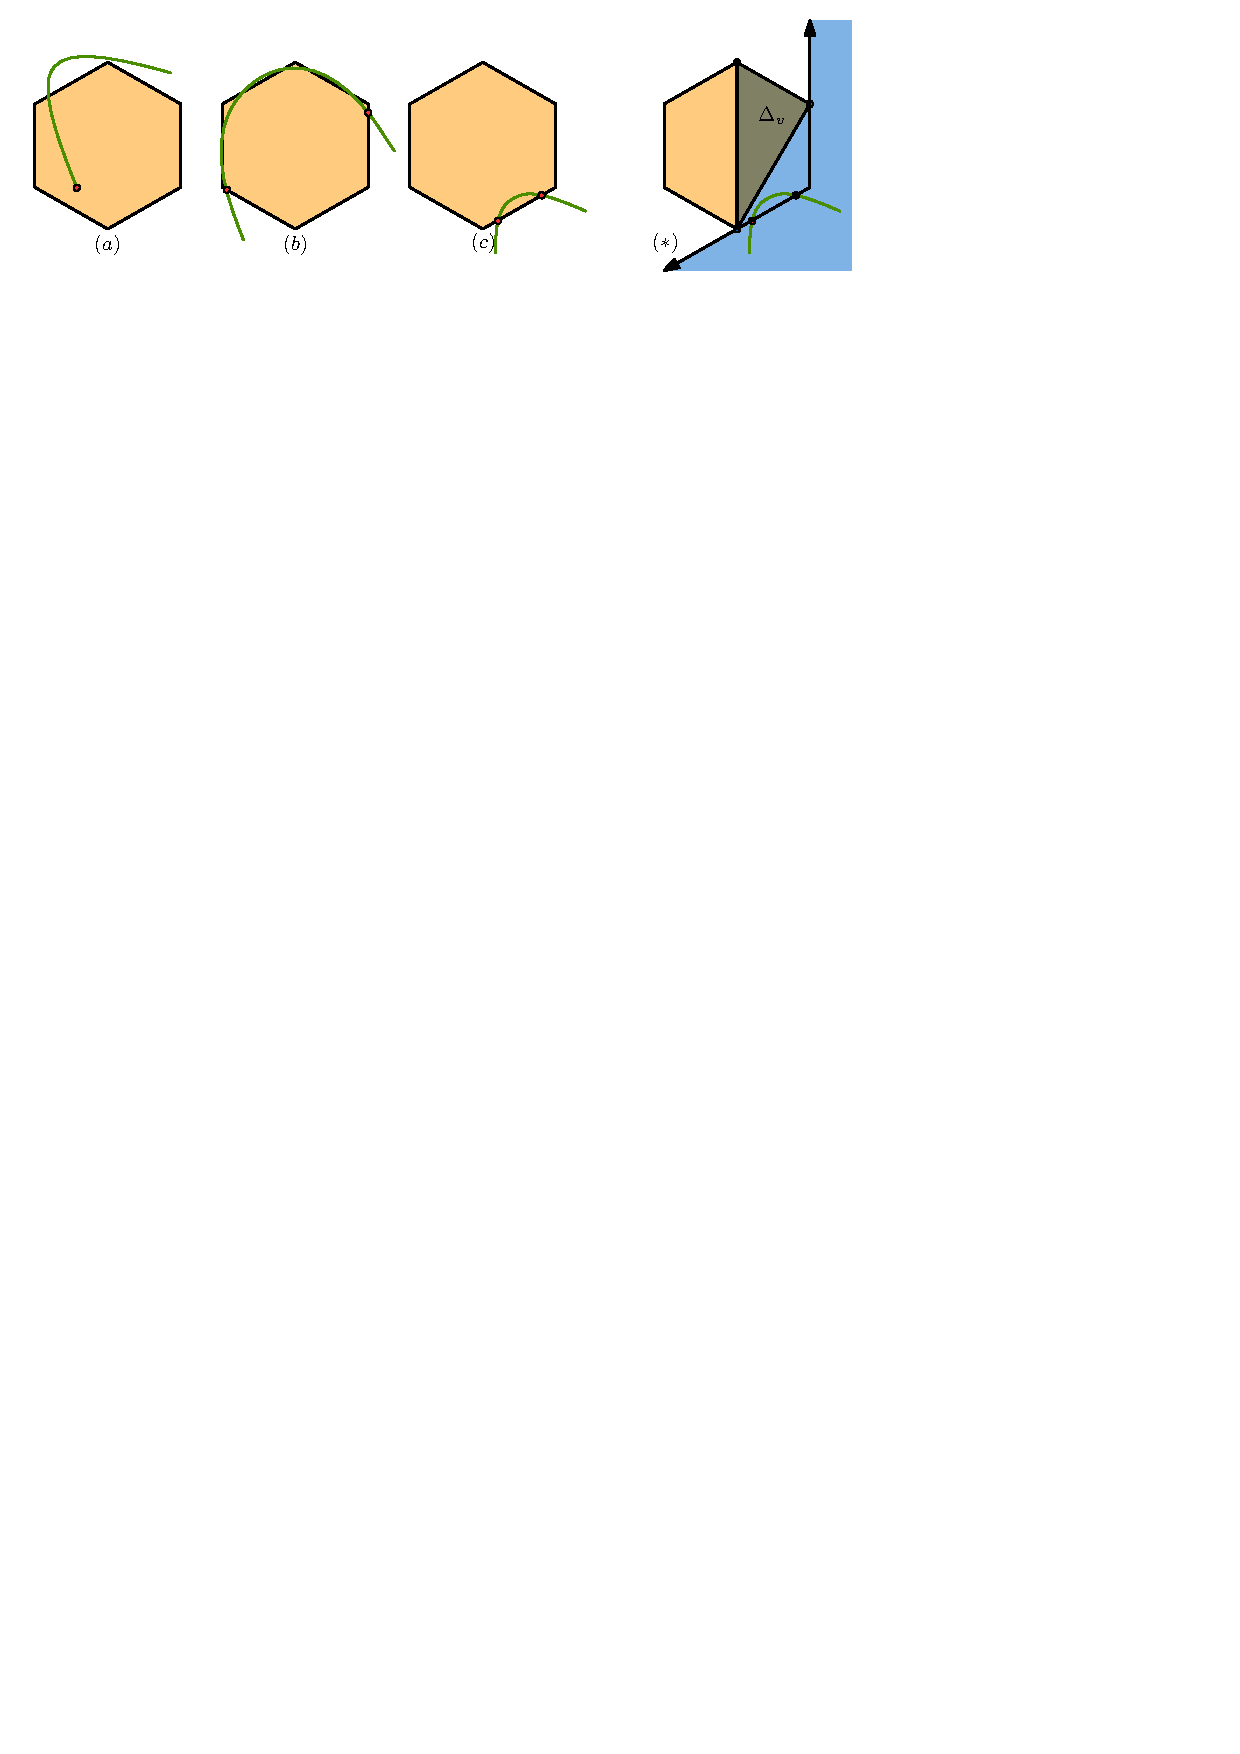
\includegraphics{../intersectionsearch}
    \caption{(left) The three cases of an intersection between $\gamma$ and $P_E$. (right) the right-subspace bound by three halfspaces.}
    \label{fig:intersectionsearch}
\end{figure}
%
\subparagraph{Intersection types (a) and (c).}
Chazelle~\cite{FRANK} shows that we can preprocess $P_E$ using $\Theta(n)$ time and space, such that point location (and thus the detection of case (a)) can be done in $\Theta(\log n)$ time. To detect an intersection of case $(c)$, we first build a hierarchical triangulation of $P_E$ using $\mathcal{O}(n)$ space and $\mathcal{O}(n)$ preprocessing time. Given $\gamma$, we recursively answer the intersection query as follows (Figure~\ref{fig:intersectionsearch} (*)): any node $v$ in this decomposition represents a sub-polygon $P'$ of $P_E$ and a triangle $\Delta_v$ which splits $P'$ in a left and right part. Consider the border of the right part $R = (e_1, e_2, \ldots, e_m)$. Note that if $\gamma$ does not intersect $\Delta_v$, then $\gamma$ can only dip an edge in $R$ if it is contained in the union of the half-spaces that lie to the right of the lines supporting (1) one edge of $\Delta_v$ and (2) $e_1$ and $e_m$ (refer to the blue area in the figure). Given the node $v$ we do three things in constant time each: first we check if $\gamma$ intersects $\Delta_v$. If not then we check for both the left and right sub-polygon if $\gamma$ is contained in the specified area. If that is the case for both or neither sub-polygons then $\gamma$ can never dip an edge of $P_E$, else we recurse. It follows that we can detect case $(c)$ in $\mathcal{O}(\log n)$ time.

\subparagraph{Intersection type (b)}

We say that the curve $\Gamma$ of which $\gamma$ is a segment divides the plane into the interior and exterior. An edge $(x_1, x_2) \times (x_3, x_4) \in E$ is intersected by $\gamma$ with an intersection of type $(b)$ only if one endpoint lies in the interior and the other in the exterior. The points $(x,y)$ on the interior of $\Gamma$ are the $(x, y)$ for which $a_1 x^2 + a_2 x + a_3 xy + a_4 y + a_5 y^2 + a_6 \le 0$. This formulation gives a straightforward linearization and transforms the question if a point $\vec{x} = (x_1, x_2)$ lies on the interior of $\Gamma$ into a halfspace range query in $\mathbb{R}^5$. 
We build a two-level data structure where the base level is a 5-dimensional halfspace range searching data structure and on top of each node we build a binary search tree on the clockwise ordering of the edges in each node.

During query time, we transform the degree-2 curve $\Gamma$ into a $5$-dimensional halfspace and obtain the edges which cross $\Gamma$ in $\mathcal{O}(Q(5))$ time represented as at most $\mathcal{O}(Q(5))$ binary search trees $T_1 \ldots T_m$. Consider the clockwise ordering of the edges in such a tree $T_i$: the subset of these edges which are intersected by the segment $\gamma$ must be a connected chain in this order. Thus (using our binary search trees on top of each node) we can obtain these consecutive chains in $\mathcal{O}(\log n)$ time for each $T_i$. The time and space needed for solving case $(b)$ dominates the time and space needed for case $(a)$ and $(c)$ and we conclude:

\begin{theorem}
    We can preprocess a simple polygon $P_E$ in $\mathcal{O}(S(5) \log n)$ and $\mathcal{O}(C(5) \log n)$ space and time, such that for any degree-2 curve segment $\gamma$ we can find if there is an intersection between $\gamma$ and at least one edge in $E$ in $\mathcal{O}( Q(5) \log^2 n)$ time. 
\end{theorem}

\section{One moving entity}
\label{sec:pointline}


In this setting we have two entities $q$ and $r$ in a polygonal domain $P$ where $q$ is stationary whilst $r$ traverses a line segment. We consider three variants of this setting: one where $P$ is a simple polygon and $r$ is contained in $P$, one where $P$ is a simple polygon and one where $P$ is a polygonal domain. In every variant we are interested in preprocessing $P$ such that given $q$ and $r$, we can determine if there is a time where $q$ and $r$ are mutually visible in sub-linear time. For reasons that will become apparent later, we say that entity $r$ walks along the line $\rho := \{ x,y \mid  0 = a_1 x - a_2 - y \}$ from a start to an end point. Entity $q$ is stationary at the point $(a_3, a_4) \in P$ and $\rho$ is parametrized such that $q$ lies below $\rho$.

\begin{figure}[h]
    \centering
    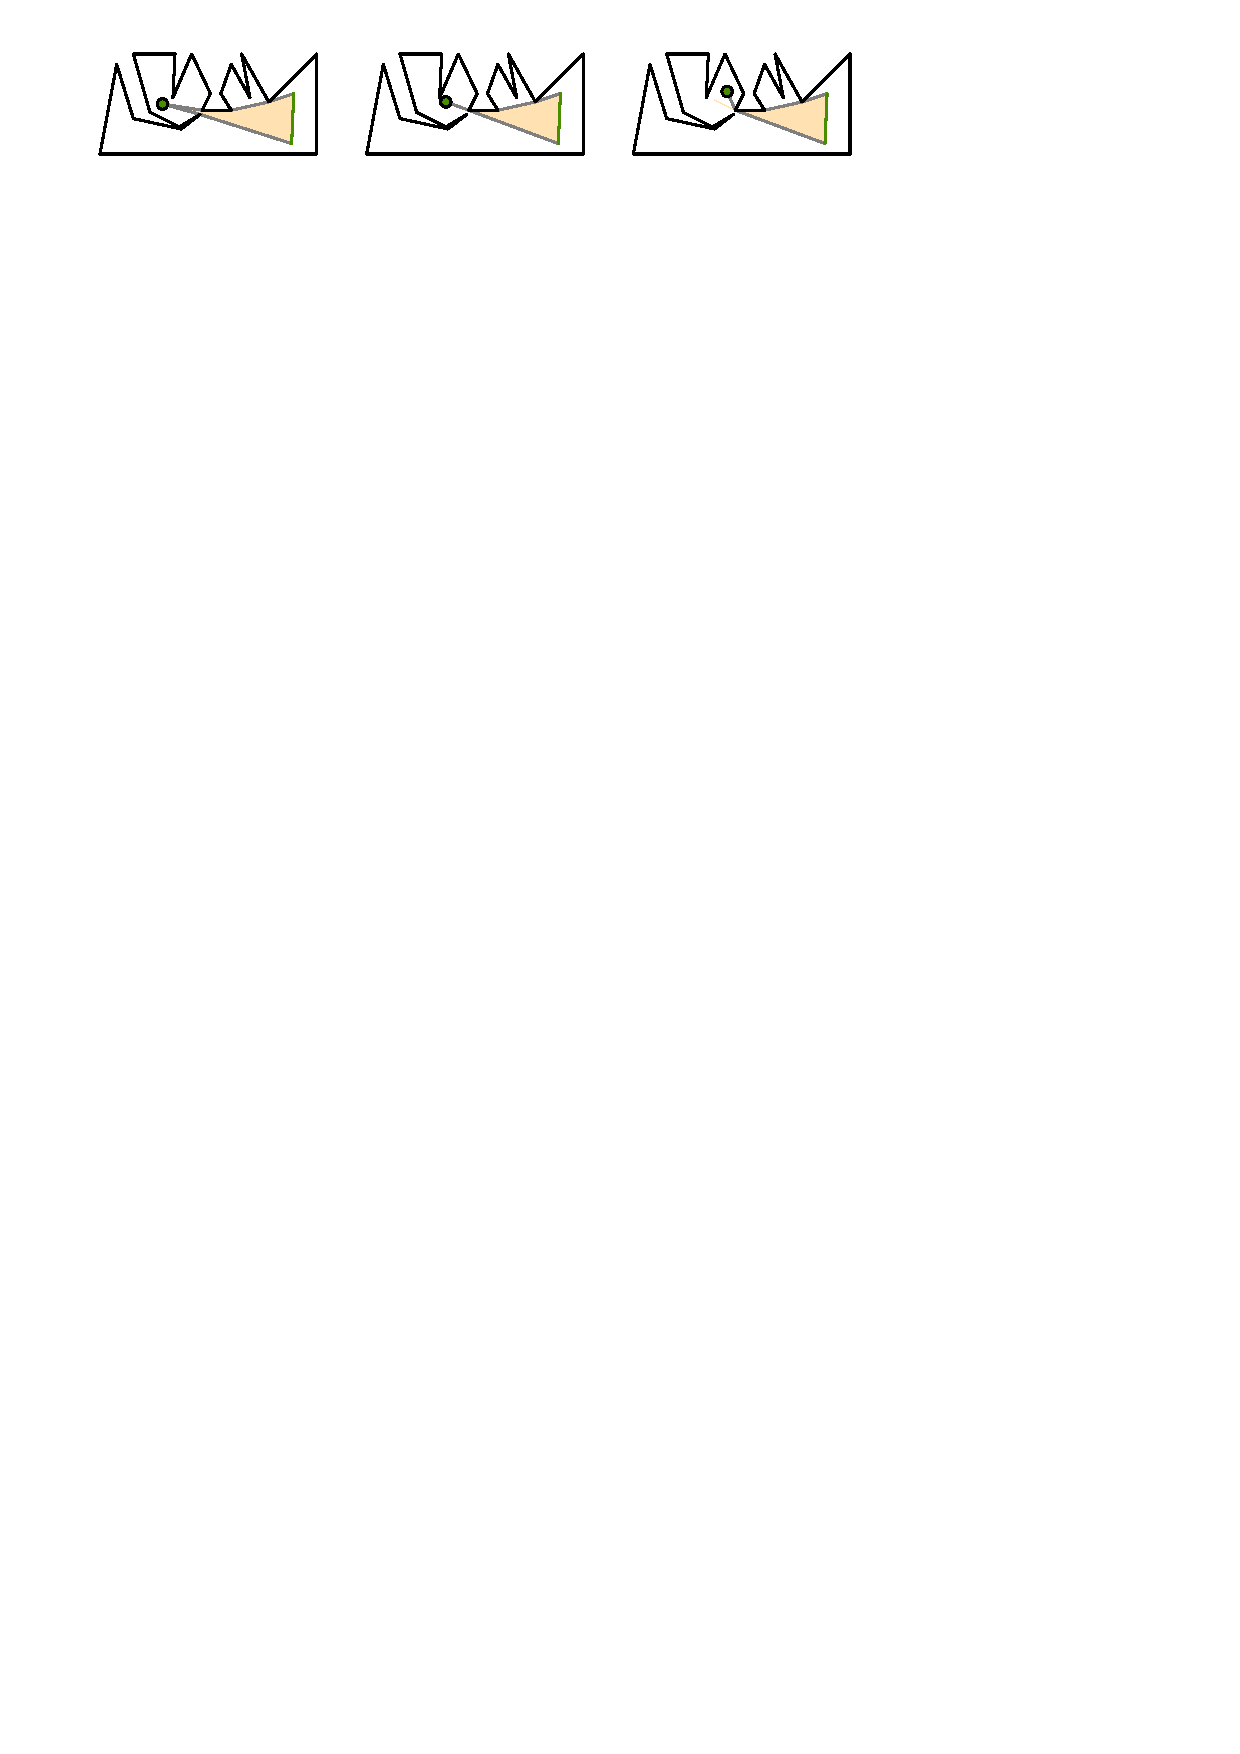
\includegraphics[]{../funnel}
    \caption{Three times a query pair $(q,r)$ in a simple polygon. In the middle case, the paths $\pi_1, \pi_2$ share their first line segment but there still is a point on $r$ which is visible from $q$.}
    \label{fig:funnel}
\end{figure}

\frank{Explain what an hourglass and a funnel are here}


\subparagraph{Entity $r$ is contained in a simple polygon.}
Consider the two shortest paths $\pi_1, \pi_2$ from $q$ to the end points of $r$. Observe that if edges of $\pi_1$ and $\pi_2$ coincide, they coincide in a connected chain from $q$. Moreover (Figure~\ref{fig:funnel}) if more than one line segment of $\pi_1$ and $\pi_2$ coincide, then any shortest path from $q$ to a point on $r$ cannot be a single line segment. If no edges of $\pi_1$ and $\pi_2$ coincide then there is at least one point on $r$, whose shortest path to $q$ is a line segment. If exactly one line segment of $\pi_1$ coincides with a segment of $\pi_2$, then that segment must be connected to $q$ and if there is a line-of-sight between $q$ and $r$, it has to follow that line segment. This observation gives us an algorithm for the visibility query in this scenario: we simply build the shortest path data structure from Guibas and Hershberger which takes $\Theta(n)$ space, has $\Theta{O}(n)$ construction and $\Theta(\log n)$ query time. Given $q$ and $r$, we use this data structure to obtain $\pi_1$ and $\pi_2$ and we check whether the first and second edge coincides. If only the first edge coincides we trace its supporting line and check if we reach $r$ without intersecting $\pi_1$ or $\pi_2$ using their binary tree representation.

\begin{theorem}
We can preprocess a simple polygon $P$ in $\Theta(n)$ space and $\Theta(n)$ time. Such that for any query point $q$ and segment trajectory $r$ which is contained in $P$, we can determine if there is a point on $r$ that is visible from $q$ in $\Theta(\log n)$ time.
\end{theorem}




\frank{integrate the thing below:}
\subparagraph{Visibility polygon retrieval.}
For any point $q$ in a polygonal domain $P$, its \emph{visibility polygon} $V_q$ is the union of all points visible from $q$. There are two types of edges bounding $V_q$ which we call fixed and variate. A fixed edge coincides with an edge of $P$. An variate edge of $V_q$ is stored as a tuple $(e, v_e)$ where $e$ is an edge and $v_e$ is a vertex of $P$. One endpoint of $e$ is the intersection between the line $qv_e$ and $e$. For all $q \in P$, the \emph{implicit} visibility polygon is a clockwise order of the fixed and variate edges of $V_q$, stored in a red-black tree. Aronov \etal \cite{aronov2002visibility} show how to partition a simple polygon $P$ into $\mathcal{O}(n^2)$ cells such that for each cell, all points in that cell have the same implicit visibility polygon. This allows them to prepreprocess $P$ in $\mathcal{O}(n^2\log n)$ time using $\mathcal{O}(n^2)$ space, such that for any query point $q$, we can get a pointer to the implicit $V_q$ in $\mathcal{O}(\log n)$ time. 
%



\subparagraph{Entity $r$ can cross a simple polygon.}
If $r$ is able to move through edges of $P$ then answering the visibility query becomes more complicated: $r$ could consist of linearly many sub-segments whose endpoints lie on the border of $P$. Inspecting each of these segments takes linear time. For any point $q \in P$, its visibility polygon $V_q$ is the union of all points which are visible from $q$. If $r$ intersects $V_q$, the point of intersection is a point on $r$ which is visible from $q$. 

In this scenario we construct a three-level data structure. The base level is from Aronov \etal who partition $P$ into $\mathcal{O}(n^2)$ cells where for each cell, all its points have the same implicit visibility polygon stored as a red-black tree. Each of these $\mathcal{O}(n^2)$ red-black trees could have linear size, so a naive implementation of the Aronov \etal data structure could take $\mathcal{O}(n^3)$ space. We first explain our data structure using this naive implementation. We then show that our secondary structures can be made partially persistent (just like the Aronov \etal data structure itself) which reduces the space requirement by a linear factor.

The implicit polygon $V_q$ could contain $\mathcal{O}(n)$ uncertain edges and depending on the location of $q$ the query segment $r$ may or may not intersect one (Figure~\ref{fig:twolevel}, middle). Consider the two rays from $q$ towards the endpoints $s$ and $t$ denote the edges of $V_q$ hit by these rays as $e_1$ and $e_2$. If $r$ intersects $V_q$ then it must intersect an edge in the consecutive chain between $e_1$ and $e_2$. The second level of our data structure finds this chain. We assumed that every triangle of the partition of $P$ contained a unique red-black tree representing an implicit visibility polygon. On top of each node in the red-black tree we build a ray shooting data structure. Ray shooting does not immediately work for any ray in $V_q$ since some edges are uncertain. However, it does work for rays originating from $q$ because each ray from $q$ per definition only stabs one edge from $V_q$.  We find $e_1$ and $e_2$ in the red black tree and with them $\mathcal{O}(\log n)$ subtrees that form our chain.

Let $T$ be a subtree returned by the second level. The root of this subtree represents a collection of $\mathcal{O}(n)$ fixed and variate edges. Denote by $U$ the set of variate edges of $T$ and by $\bar{U}$ the fixed edges. We build two separate data structures on top of $T$ that search for an intersection between $r$ and an edge in $\bar{U}$ or $U$ respectively. The data structure on $\bar{U}$ is the ray shooting data structure that we mentioned above. If a ray from the start of $r$ to end of $r$ hits a certain edge, we know that we found a point on $r$ that can see $q$. The data structure on $U$ is an $8$-dimensional halfspace range \emph{emptyness} structure: 

\begin{lemma}
\label{lemma:uncertain_intersection}
For each edge $e \in U$, there is a unique 8-dimensional point, such that for each query pair $(q, r)$ there is a unique $8$-dimensional halfspace, such that $r$ intersects $e$ if and only if the point of $e$ is in that halfspace.
\end{lemma}

\begin{figure}[h]
    \centering
    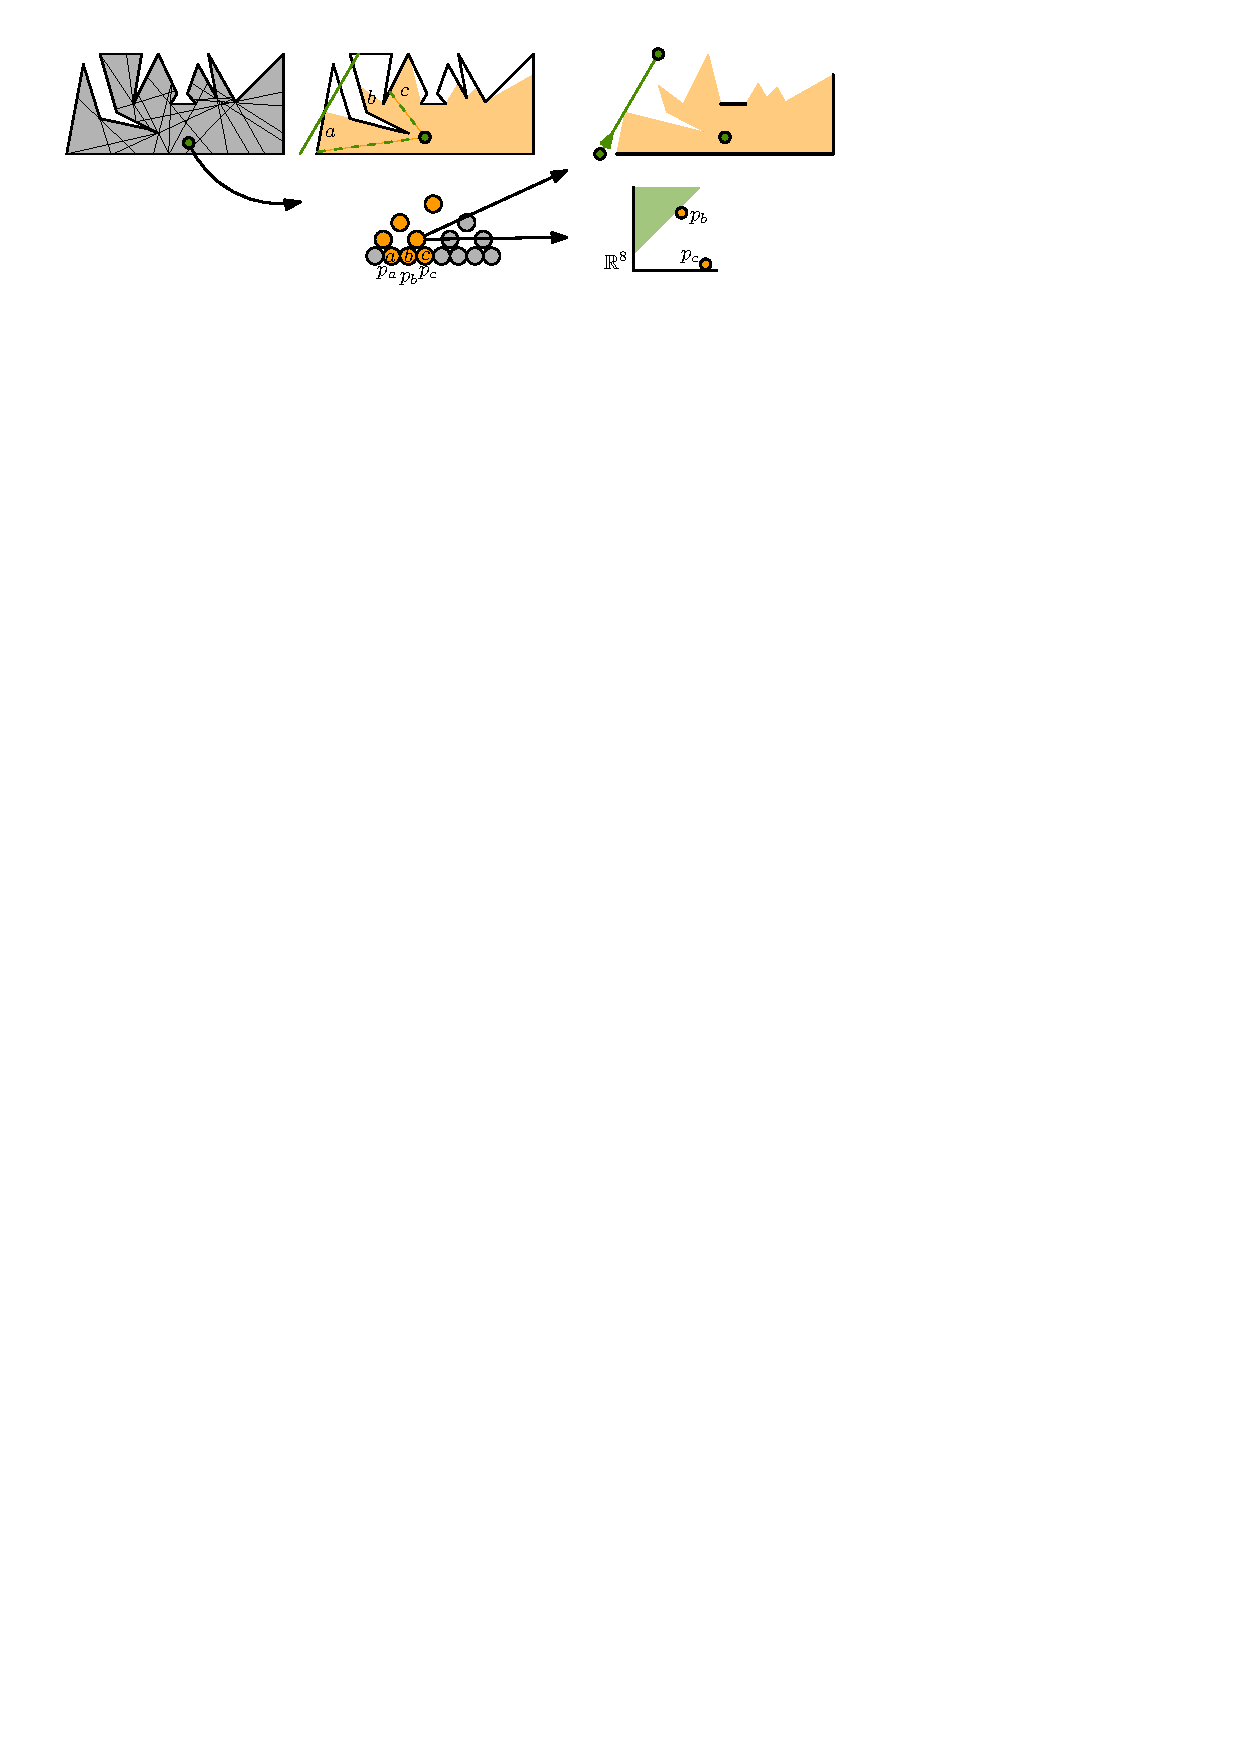
\includegraphics[]{../twolevel}
    \caption{ (left) A simple polygon split in $\mathcal{O}(n^2)$ cells. For each cell, there exists a red-black tree that represents a visibility polygon. (middle) Given $V_q$ and $r$, $r$ could intersect the explicit $V_q$ depending on the location of $q$. We shoot two rays from $q$ to $r$ and find their intersection with $V_q$ in the red-black tree. That gives us three leaves highlighted in orange. (right top) All the fixed edges in this node are stored in a ray-shooting data structure, (right bottom) all the variate edges have 8-dimensional points that are stored in an $8$-dimensional partition tree.}
    \label{fig:twolevel}
\end{figure}

Our final data structure (Figure~\ref{fig:twolevel}) looks as follows: let $\Delta_q$ be a triangle in $P$ representing an implicit visibility polygon $V_q$. To each uncertain edge of $V_q$ we assign an $8$-dimensional point. $\Delta_q$ stores a red-black tree and for each node in this tree we do two things: (1) we identify the uncertain edges in this node and we build an $8$-dimensional partition tree on their corresponding points, (2) we identify the certain edges and build a ray shooting data structure on these points.
$8$-dimensional partition trees on $m$ points take $\mathcal{O}(n)$ space and can be constructed in $\mathcal{O}(n^{3/4})$ time and this dominates the time and space requirement for the ray shooting data structure. Each edge of $V_q$ occurs in at most $\mathcal{O}(\log n)$ nodes and thus two-level data structure in $\Delta_q$ takes up at most $\mathcal{O}(n \log n)$ space per triangle $\Delta_q$.

At query time we first find the triangle $\Delta_q$ containing $q$ in $\mathcal{O}(\log^2 n)$ time. The secondary layer identifies at most $\mathcal{O}(\log n)$ subtrees in $\Delta_q$ which together for the relevant portion of the border of $V_q$. Given $r$ and $q$, we compute an $8$-dimensional halfspace query range in constant time and we query the partition trees of each of these $\mathcal{O}(\log n)$ trees in $\mathcal{O}(n^{3/4})$ time which dominates the earlier time used to find $\Delta_q$. There is an intersection between $r$ and an uncertain edge of $V_q$ if and only if at least one of these query ranges is non-empty.  Thus we can conclude:


% \subparagraph{Persistence.}
% The aforementioned data structures create a hierarchical decomposition of $P$ and store in each node of this tree an implicit representation of a sub-polygon of $P$ (be it an hourglass or a visibility polygon) as a red-black tree. A persistent data structure (introduced by Sarnak and Tarjan \cite{sarnak1986planar}) is a data structure that accepts an arbitrarily long sequence of updates, but is able to remember at any time all its earlier versions. Both data structures make use of persistence to save storage space \cite{hershberger1991new, aronov2002visibility}: instead of storing a unique tree at every node of the decomposition they store one partially persistent red-black tree  which for each adjacent node in the decomposition, remembers an update that transforms the red-black tree into the node for that tree.
% %

\subparagraph{Saving Space} Use persistence here.

\frank{TODO}



\begin{theorem}
  We can preprocess a simple polygon $P$ in $\mathcal{O}( n^3 \log n)$ space and \\ $\mathcal{O}(n^3 \log n)$ time. Such that for any query point $q$ and segment trajectory $r$, we can determine if there is a point on $r$ that is visible from $q$ in $\mathcal{O}(n^{3/4} \log n)$ time.
\end{theorem}




\subparagraph{Polygonal domains, persistence with transient updates.}

\frank{TODO}

Frank proves that $n^2$ is really $n^2$ and not $n^3$. Moreover, Vegter and Pol-whatever exist for polygonal domains.


\section{Line-Line}
\label{sec:lineline}


In this setting we have two entities $q$ and $r$ in a polygonal domain $P$ which both traverse a line segment, possibly at different (constant) speeds, during the time interval $t \in [0,1]$. We investigate three variants of this setting: one where $P$ is a simple polygon and $q$ and $r$ are contained in $P$, one where $P$ is a simple polygon and one where $P$ is a polygonal domain. We say that $q$ walks from the point $(a_1, a_2)$ to $(a_1 + a_3, a_2 + a_4)$ and $r$ walks from the point $(a_5, a_6)$ to $(a_5 + a_7, a_6 + a_8)$. 
\begin{figure}[t]
    \centering
    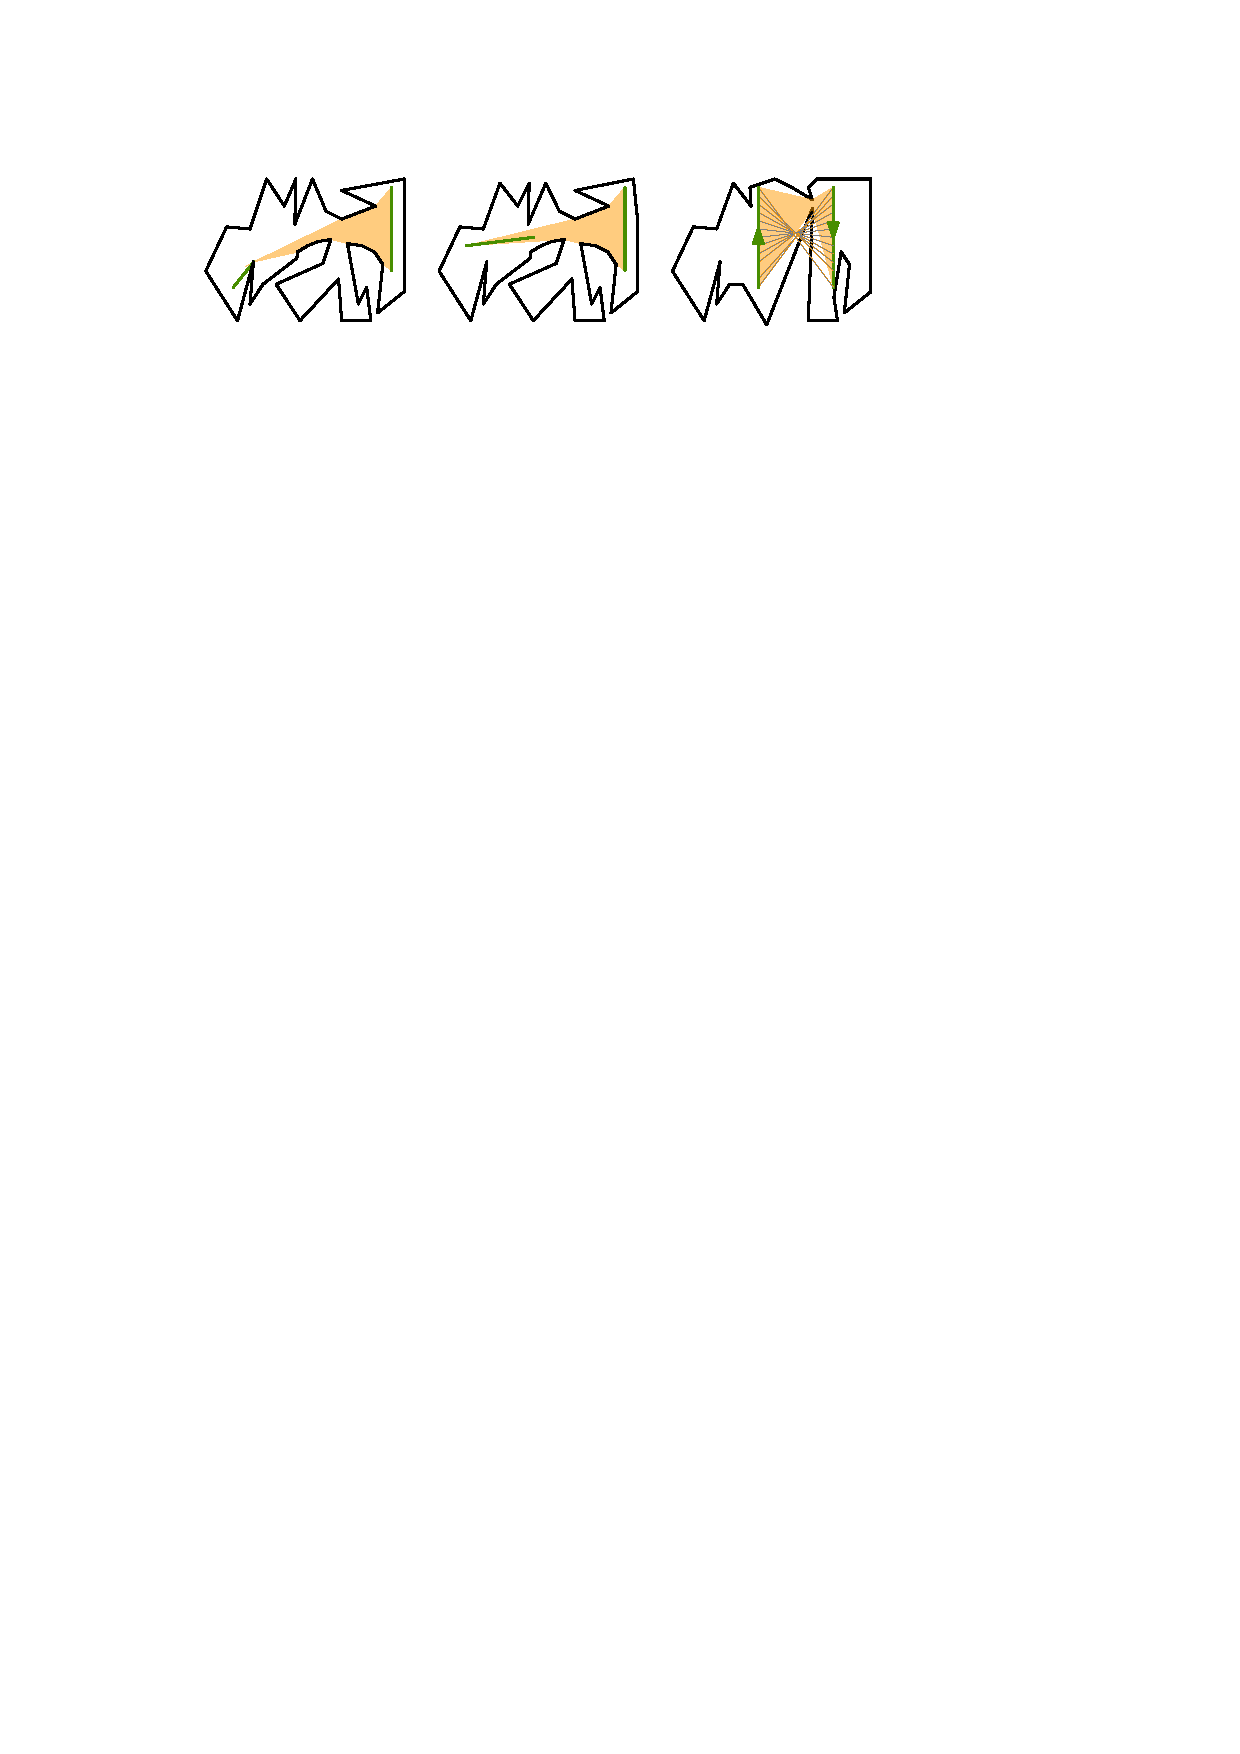
\includegraphics[]{../edgecase}
    \caption{(left + middle) Two placements of $q$ and $r$ that realise a funnel. (right) $L(q,r)$ is clearly non-empty but there is never a time where $q$ and $r$ are mutually visible. }
    \label{fig:edgecase}
\end{figure}


\frank{integrate this here somewhere}
\subparagraph{Shortest path queries.}
Given a simple polygon with $n$ vertices, Guibas and Hershberger \cite{guibas1989optimal} create a $\Theta(n)$ size data structure, in $\Theta(n)$ time, that for any two points $q$ and $r$ can return shortest-path queries in $P$ in $\Theta(\log n + l)$ time where $l$ is the length of the path. They build a balanced hierarchical subdivision~\cite{FRANK} of $P$ using its diagonals, where the leaves in the subdivision form a triangulation of $P$.
Let $e$ and $e'$ be two edges in $P$, the \emph{hourglass} $H(e, e')$ is the union of all shortest paths from points on $e$ to points on $e'$. $H(e, e')$ is a polygon in $P$ which is bound by $e, e'$ and the shortest paths between the endpoints of $e$ and $e'$. Since an hourglass is bounded by four paths in $P$, the hourglass can be represented as a red-black tree where each node represents an edge on the border of $H(e, e')$, this is called the \emph{implicit representation}. Each node in the hierarchical decomposition stores several implicit hourglasses between diagonals. At query time, Guibas and Hershberger locate the leaf triangles $\Delta_q$ and $\Delta_r$ which contain the query points $q$ and $r$. They identify  $\mathcal{O}(\log n)$ pre-stored hourglasses and concatenate them using at most $\mathcal{O}(\log n)$ \emph{outer tangents} to form the hourglass between $\Delta_q$ and $\Delta_r$. This hourglass can be used to find the shortest path between $q$ and $r$. Refer to Figure~\ref{fig:guibas} for an example. 
%
\begin{figure}[h]
    \centering
    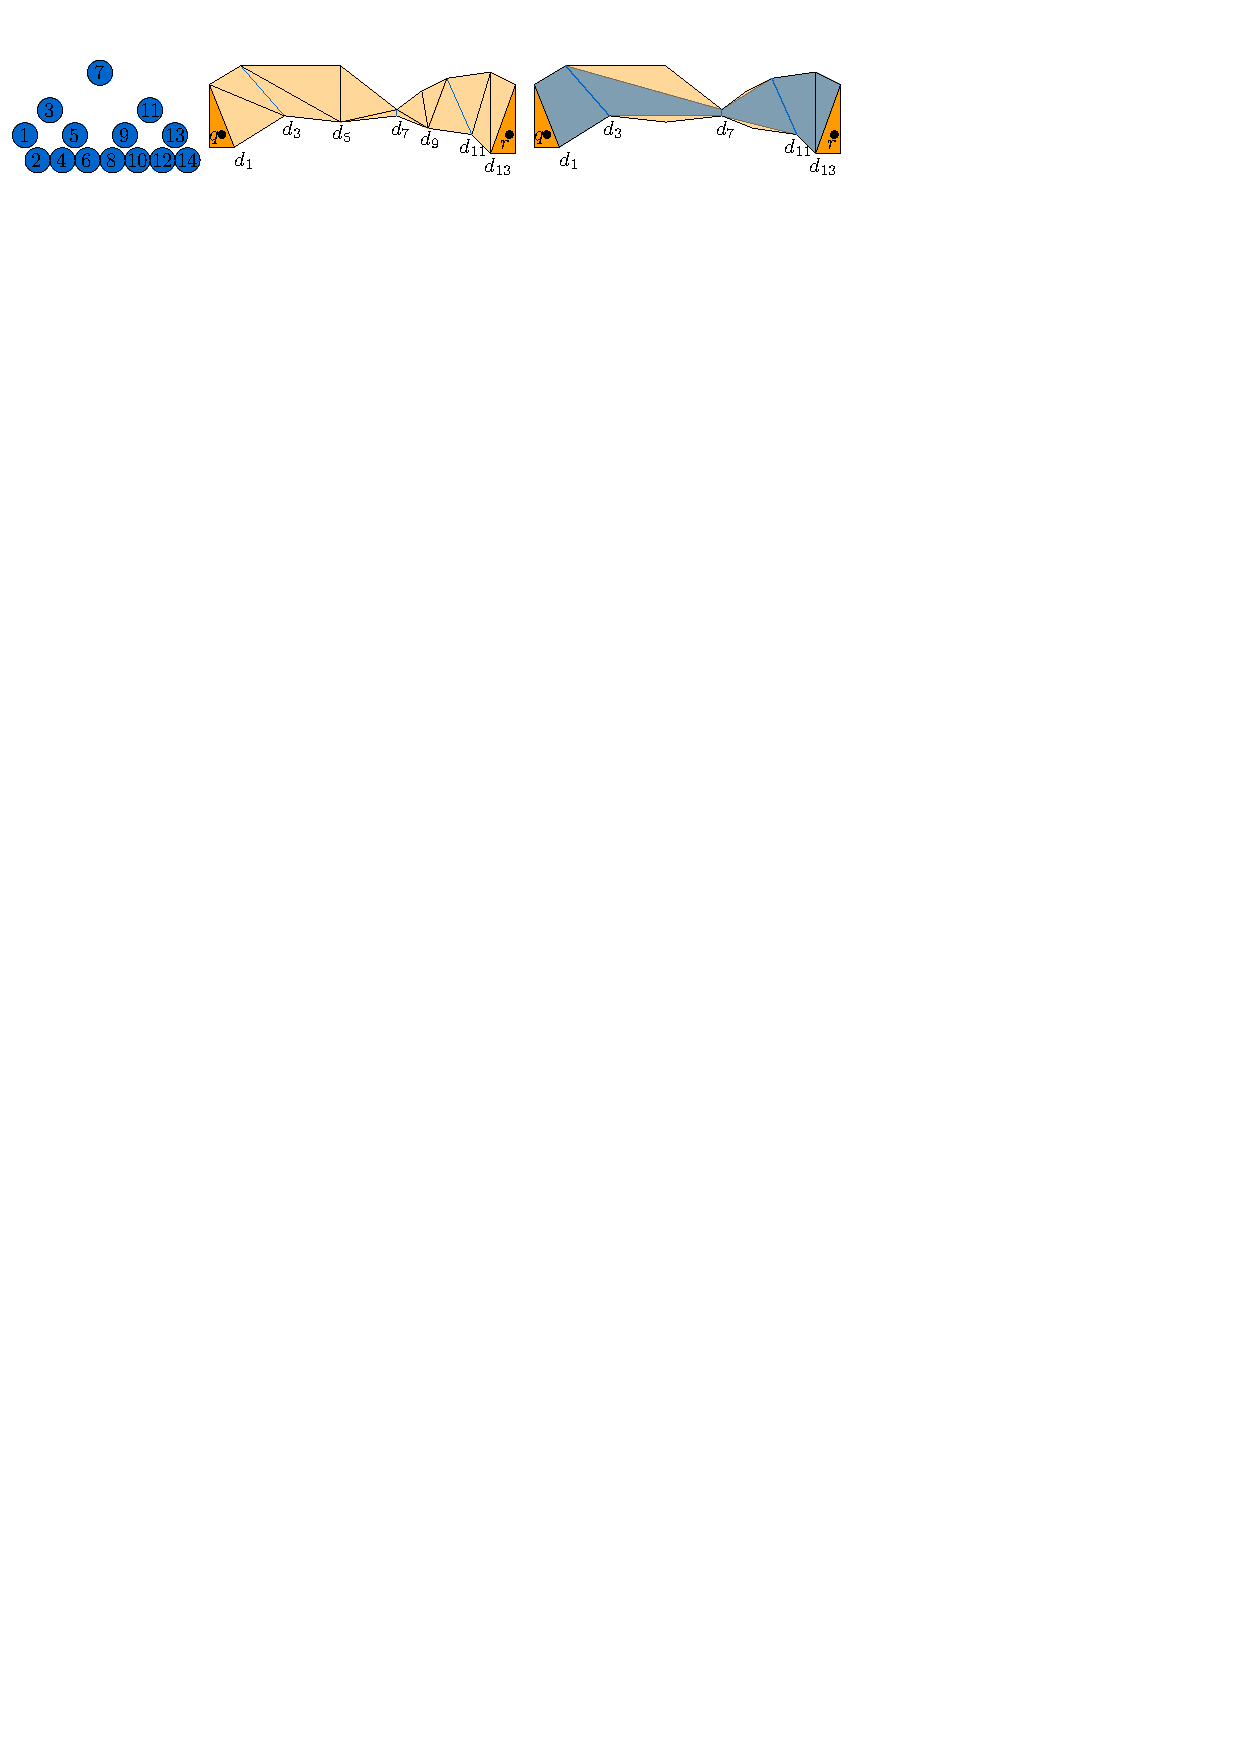
\includegraphics[]{../guibas}
    \caption{A triangulated polygon $P$ where the diagonals are labelled from $d_1$ to $d_{14}$. (left) a balanced hierarchical subdivision on the diagonals. (right) There are $13$ diagonals between $\Delta_q$ and $\Delta_r$. However, we have pre-stored hourglasses $H(d_1,d_3)$, $H(d_3, d_7)$, $H(d_7, d_{11})$ and $H(d_{11}, d_{13})$. Thus during query time, we only have to concatenate $\mathcal{O}(\log n)$ hourglasses to get $H(d_1, d_{13})$. }
    \label{fig:guibas}
\end{figure}

\subparagraph{The entities are contained in a simple polygon.}
The hourglass $H(q, r)$ is the union of all the shortest paths between $q$ and $r$. 
Recall that $H(q,r)$ is a polygon bound by the shortest paths between the endpoints from $q$ and $r$ together with $q$ and $r$ itself. There is a special case illustrated in Figure~\ref{fig:edgecase} for $H(q,r)$ which is when $q$ has one endpoint which is the furthest point on $q$ from all points on $r$ (or vice versa). We call this case a \emph{funnel}. If $H(q,r)$ is a funnel, then Section~\ref{sec:pointline} shows how to compute visibility.

The hourglass $H(q, r)$ could contain many shortest paths which are not line segments and therefore not candidate line-of-sights between the two entities. We define the \emph{visibility glass} $L(q,r)$ as the collection of line segments between $q$ and $r$ that are contained in $P$. $L(q,r)$ is a subset of $H(q,r)$ and could be empty. If $L(q,r)$ is empty then $q$ is never visible from $r$, but the converse is not necessarily true (Figure~\ref{fig:edgecase}). We check if there is a time where the two entities are mutually visible, through testing if there is a time where the line segment between them lies in $L(q,r)$ using the following Lemma:

\begin{lemma}[Follows from Lemma 2.1 \cite{Chazelle1989}]
For any two segments $q, r \in P$, there exist segments $q' \subset q, r' \subset r$ s.t. $V(q, r) = H(q', r')$. Moreover, $q'$ and $r'$ are bound by the bitangents of $H(q, r)$.
\end{lemma}

If $H(q,r)$ is not a funnel then $H(q,r)$ is bouned by $q, r$ and two semi-convex subchains (which we refer to as the upper and lower chain) that end in upper and lower endpoints of $q$ and $r$. Consider the shortest path $\pi$ from the upper point of $q$ to the lower point of $r$. $\pi$ partially coincides with the upper and lower chain, and its two coinciding paths are joined by a single line segment. The extension of this line segment is the bitangent of $H(q,r)$~\cite{FRANK}. Since the upper and lower chain are convex chains, this bitangent segment is the only segment on $\pi$ that starts with a clockwise and ends with a counter-clockwise rotation. 


\begin{figure}[h]
    \centering
    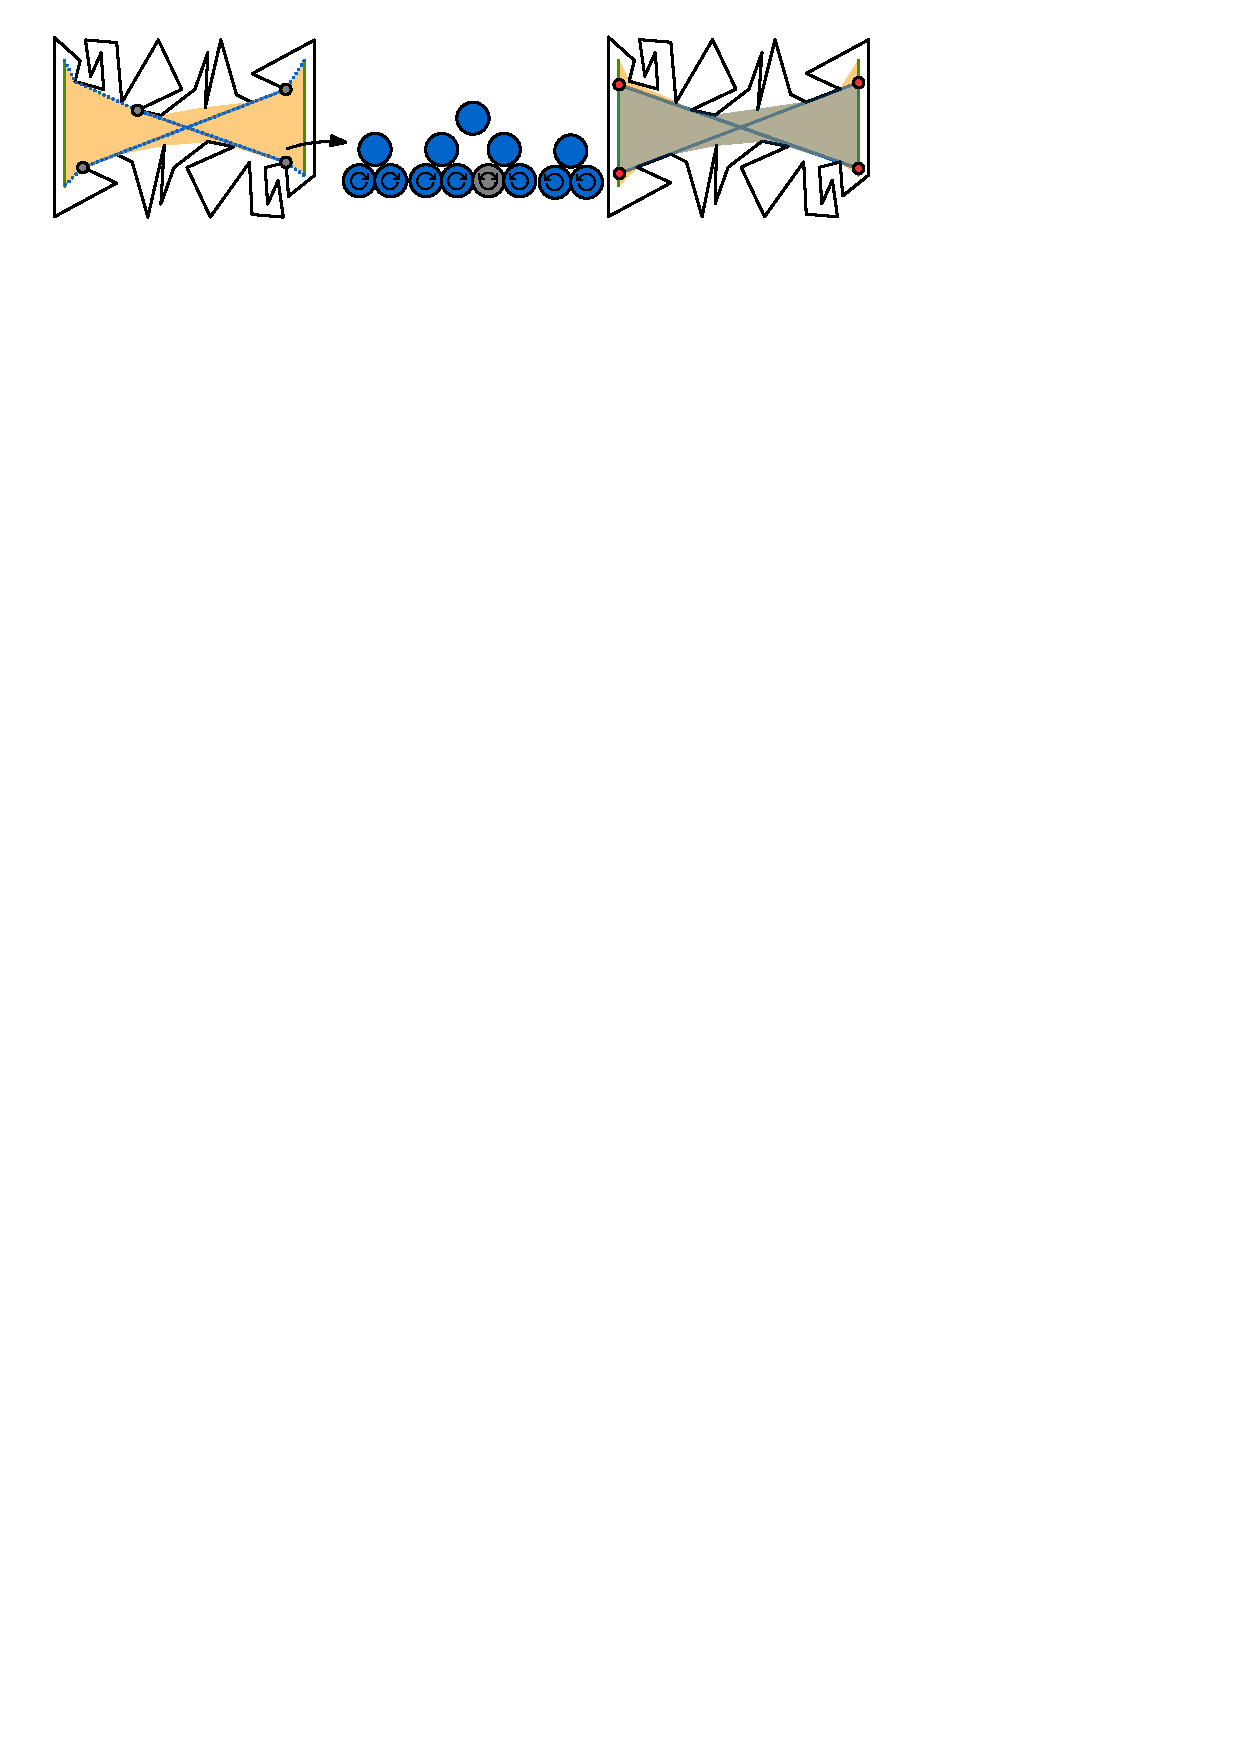
\includegraphics[]{../visibilityglass}
    \caption{(left) $H(q,r)$ in orange with the shortest paths between endpoints in dotted blue. The bitangents are underlined in grey. (middle) We obtain each dotted path as a collection of binary search trees, where only the bitangent starts in clockwise and ends in counterclockwise rotation. (right) Using the bitangents, we identify the endpoints of $q'$ and $r'$ and obtain $L(q,r)$ in grey. }
    \label{fig:visibilityglass}
\end{figure}

Using this information we can obtain the visibility glass $L(q,r)$ using the data structure $\mathcal{D}$ from \cite{guibas1989optimal} (refer to Figure~\ref{fig:visibilityglass}). Given $q$ and $r$, we can obtain the border of $H(q,r)$ as a set of $\mathcal{O}(\log n)$ concatenated persistent red-black trees. We can binary search these trees to detect if $H(q,r)$ is a funnel. If $H(q,r)$ is not a funnel, we can find the two bitangents of $H(q,r)$ as follows: we query $\mathcal{D}$ for the path $\pi$ from the upper point of $q$ to the lower point of $r$ and obtain this path as a set of $\mathcal{O}(\log n)$ red-black trees. We perform a binary search on these trees to locate the bitangent segment that starts with a clockwise and ends with a counter-clockwise rotation. We perform a symmetrical procedure to identify the second bitangent.
These two bitangents bound the segments $q'$ an $r'$. We query $\mathcal{D}$ one more time with these two segments to obtain $H(q', r') = L(q,r)$ in its implicit representation. Each query in $\mathcal{D}$ takes $\mathcal{O}(\log n)$ time and so does our binary search thus we conclude:

\begin{lemma}
\label{lemma:visibilityquery}
  The Guibas and Hershberger data structure can for any segment $q,r$ contained in $P$ obtain the implicit representation of $L(q,r)$ in $\mathcal{O}(\log n)$ time.
\end{lemma}

 
Given $L(q,r)$, we want to test if there is ever a time $t^*$ where the segment between the two entities lies in $L(q,r)$. A line segment coincides with a line segment in $L(q,r)$ if and only if their extended lines coincide. Chazelle and Guibas \cite{Chazelle1989} note, that if we dualise the collection of all lines through $L(q,r)$ then we obtain a convex polygon denoted by $\Lambda(q,r)$ of linear complexity. The line through the two entities coincides with a line in $L(q,r)$ if and only if its dualized point lies in $\Lambda(q,r)$. We detect such a point using Lemma~\ref{lemma:hyperbola}. 
At this point we have transformed the visibility query in the primal to an intersection query between a convex polygon and a degree-2 curve segment in the dual and we implore our data structure from Section~\ref{sec:intersectionsearch}. In its general form, this data structure transforms an intersection query between an arbitrary degree-2 curve segment into a halfspace emptyness query in $\mathbb{R}^5$. Our query segment has one fewer degree of freedom than a general degree-2 curve which immediately makes it a halfspace emptyness query in $\mathbb{R}^4$ instead (refer to Equation~\ref{eq:hyperbola}).

\begin{lemma}
\label{lemma:hyperbola}
  The continuous dualization of the line through the two entities, traces a degree-2 curve segment $\gamma$ for $t \in [0,1]$ with five degrees of freedom.
\end{lemma}


\begin{figure}[h]
    \centering
    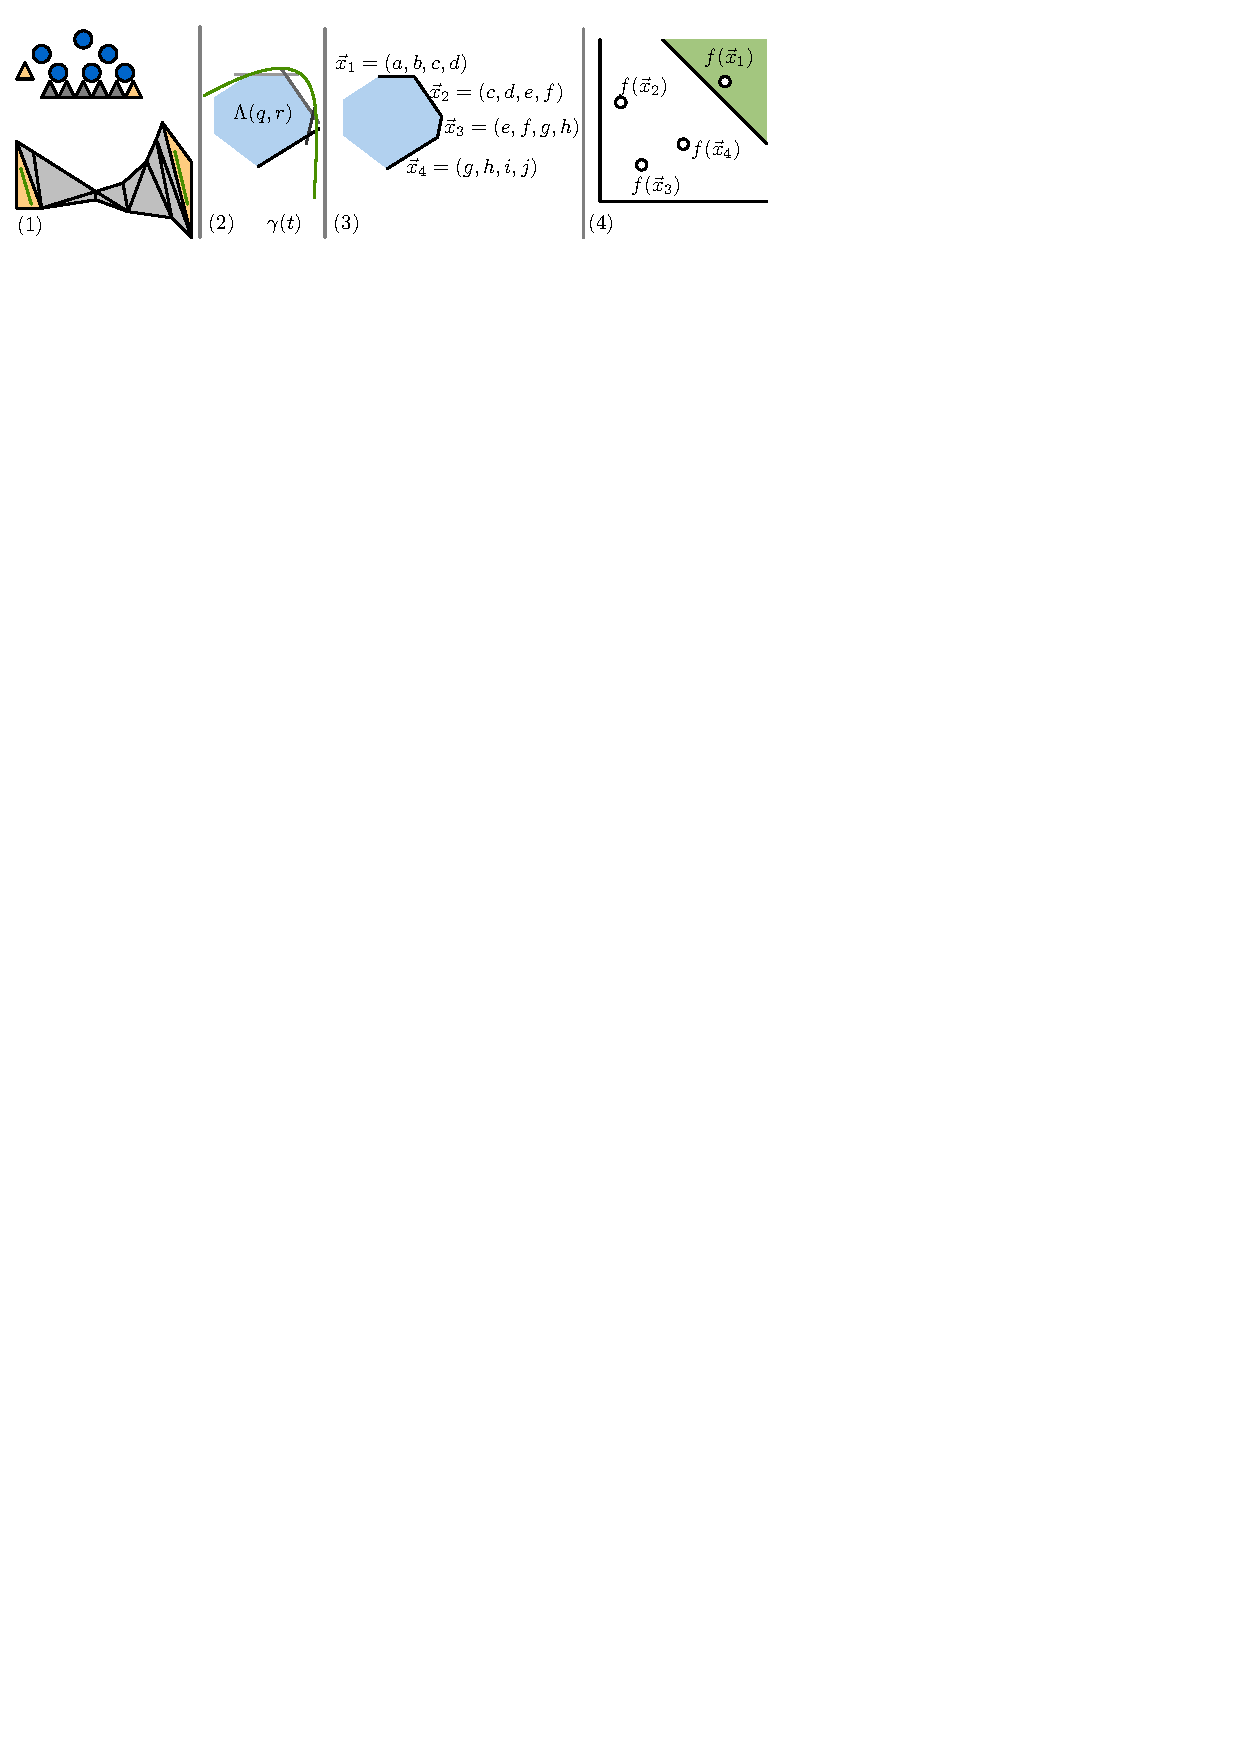
\includegraphics[]{../panel}
    \caption{(1) The base level of our data structure is a hierarchical triangulation. (2) Given $q$ and $r$, we compute $\Lambda(q,r)$ and the degree-2 query curve $\gamma$. (3) We store the parameters of each edge of $\Lambda(q,r)$ (4) Each parameter vector gets mapped to a point in $\mathbb{R}^4$ and the query curve segment gets mapped to a 4-dimensional halfspace which is empty only if $\gamma$ intersects no edge from $\Lambda(q,r)$.}
    \label{fig:panel}
\end{figure}


Our final data structure (Figure~\ref{fig:panel}) is a two-level data structure with some interesting technicalities. The base level is the hierarchical decomposition $\mathcal{D}$ of $P$. The leaves of this tree represent a triangle in a triangulation of $P$ and every node in the tree stores the dual of constantly many hourglasses (which may be an unbounded region), represented as a red-black tree on its edges. Every vertex of $P$ in the primal, is contained in at most $\mathcal{O}(\log n)$ of these pre-stored hourglasses \cite{FRANK} so our naive implementation of this data structure takes $\mathcal{O}(n \log n)$ space. \footnote{something about not using persistence}
Every pre-stored hourglass represts a collection of line segments and each line segment has a unique representative point in $\mathbb{R}^4$. In the second level of our data structure we store the representative points in the two-level data structure from Section~\ref{sec:intersectionsearch}. This (4-dimensional) data structure can store $m$ points in $S(4) \log n$ space. Thus, the final data structure uses $\mathcal{O}(S(4) \log^2 n)$ space.

\subparagraph{Querying.}
When we get $r$ and $q$ we have to decide if there exists
a time $t^*$ at which $r$ and $q$ are mutually visible. We can compute the query segment $\gamma$ in constant time. Using Lemma~\ref{lemma:visibilityquery} we obtain the implicit representation of $\Lambda(q,r)$ (the dual of the visibility glass) in $\mathcal{O}(\log n)$ time. Recall that $L(q,r)$ is the concatenation of $\mathcal{O}(\log n)$ hourglasses: that is $L(q,r)$ is a collection of $\mathcal{O}(\log n)$ inward-convex chains $C_0 \ldots C_m$ (which are stored in a subtree of a red-black tree), each joined by an outer tangent $\tau_1 \ldots \tau_{m}$. Refer to Figure~\ref{fig:chain} for an example. The dual of $L(q,r)$ is a concatenation of the dual of each inward-convex chain $C_0 \ldots C_m$ where each two chains $C_{i-1}, C_{i}$ are joined by a vertex which is the dual of $\tau_i$. 

Given the implicit representation of $\Lambda(q,r)$, we would like to immediately search for an intersection and the query curve $\gamma$ however a slight technicality appears: Consider the dualization of an inward-convex chain $C_i$ with respect to the polygon $\Lambda(q,r)$: $\Lambda(q,r)$ contains a subset of this chain, which is cut off by two outer-tangents which were not known before query time. These cut-off points were constructed during the query from $\cite{guibas1989optimal}$. During that query we can remember a pointer to each of the $\mathcal{O}(\log n)$ cut-off points induced by the outer-tangents. The result is, that the border of $\Lambda(q,r)$ is represented by at most $\mathcal{O}(\log n)$ red-black trees, which are bound by $\mathcal{O}(\log n)$ nodes induced by the outer tangents. The leaves of these trees are fixed vertices in $P$ (and therefore fixed edges in $\Lambda(q,r)$) and in the dual these fixed edges are joined by at most $\mathcal{O}(\log n)$ edges which we discover at query time.
%
\begin{figure}[h]
    \centering
    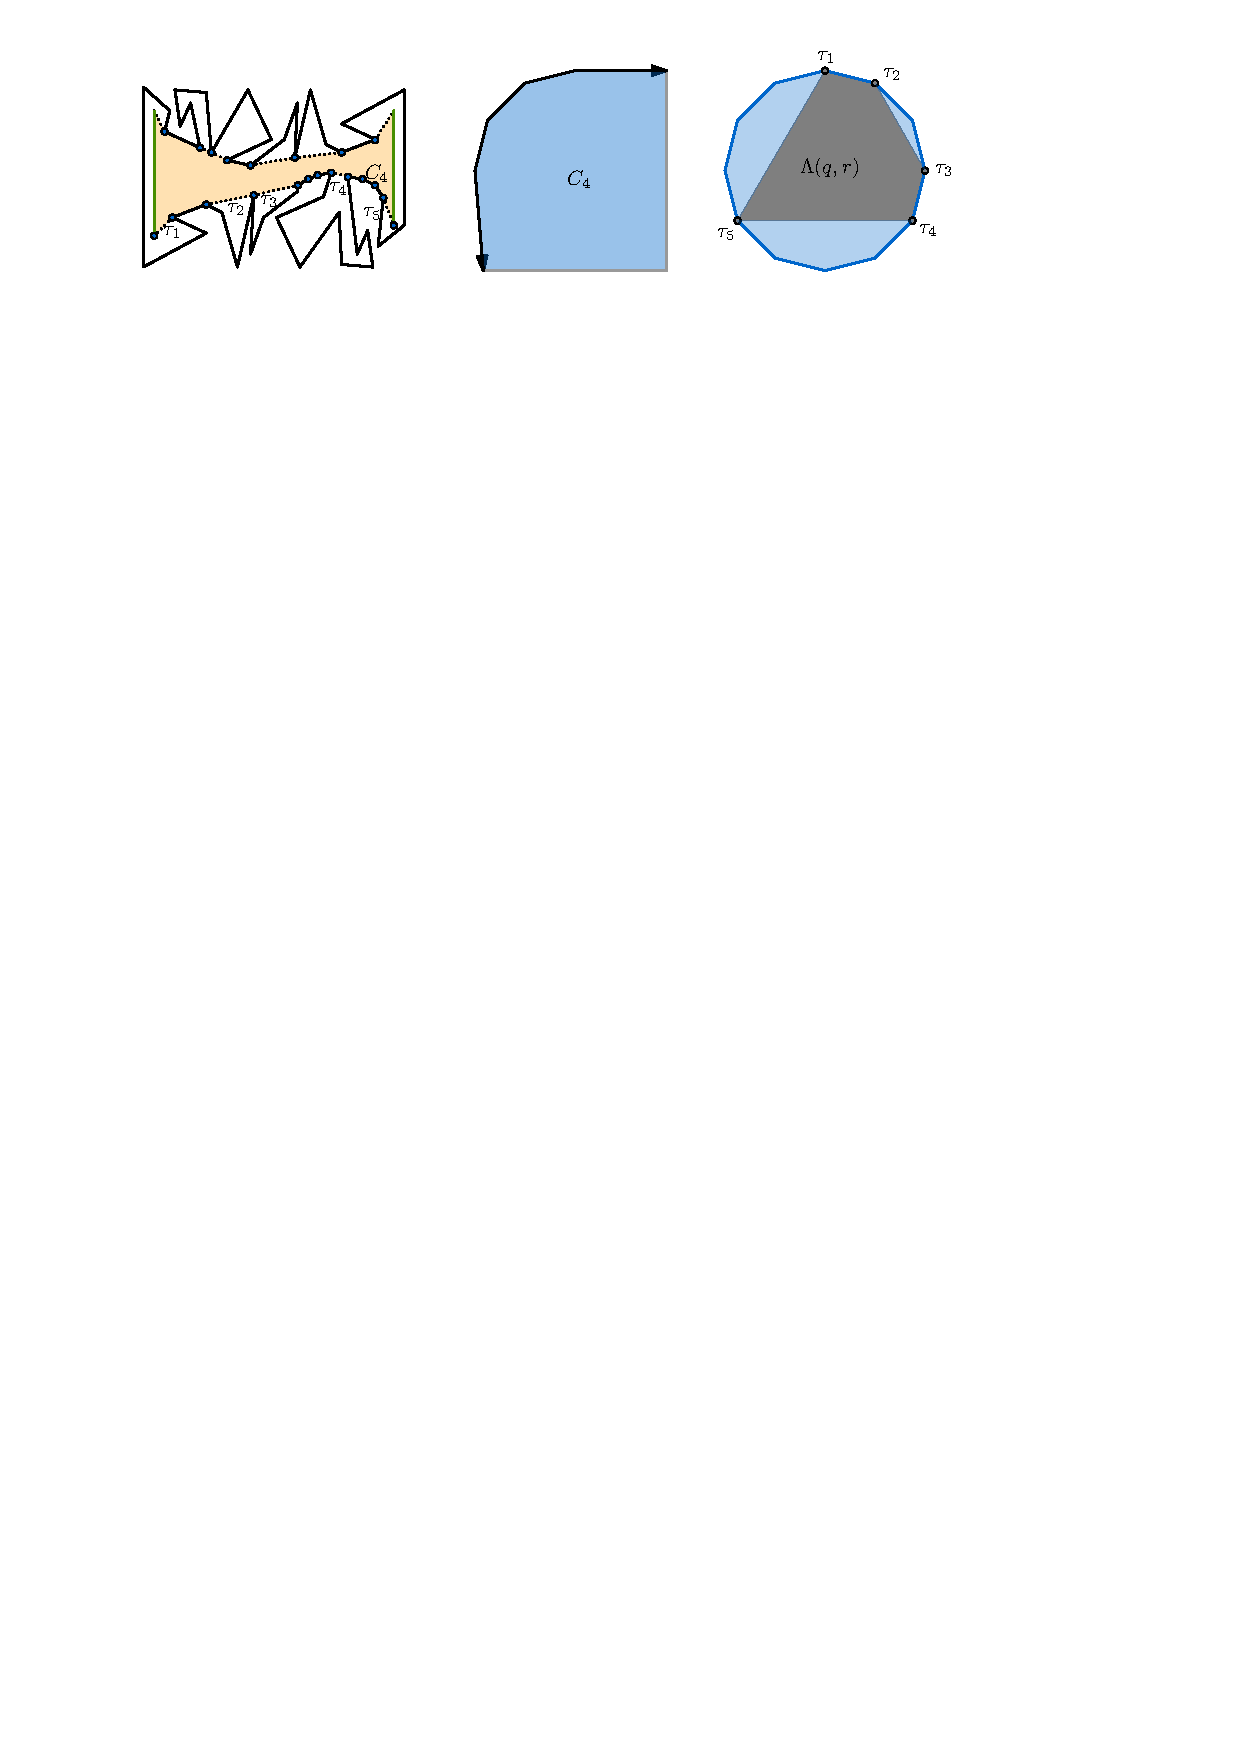
\includegraphics[]{../chain}
    \caption{(left) An hourglass between $q$ and $r$ in orange. The lower chain consists of five chains which coincide $P$ that are joined by outer tangents in dotted lines labelled $\tau_1 \ldots \tau_5$. (middle) An example of an area bound by the dualized chain $C_4$. (right) A simplified version of $\Lambda(q,r)$. Note that outer tangents could become vertices of $\Lambda(q,r)$.}
    \label{fig:chain}
\end{figure}
%
Being aware of this technicality we proceed as follows: we manually check if any of the $\mathcal{O}(\log n)$ uncertain edges intersect our query curve segment. If not, we have $\log n$ pre-stored trees where each tree represents a chain bordering $\Lambda(q,r)$. Recall that in Section~\ref{sec:intersectionsearch} we observed that a degree-2 curve segment can intersect a polygon in 3 cases labelled (a), (b) and (c). The argument for cases (b) and (c) still holds, but any subtree tree $T$ found by the base level of our data structure bounds a convex area which is larger than its portion on $\Lambda(q,r)$. However, observe the following: suppose an endpoint of the query segment lies within $\Lambda(q,r)$, in our application this means that either the two start points of $q$ and $r$, or the two end points of $q$ and $r$ are mutually visible. Checking if these two points are visible in the primal, can easily be done in logarithmic time. It follows that we can test for an intersection between our query curve segment and $\Lambda(q,r)$ in $Q(4) \log n$ time.

\begin{theorem}
    We can preprocess a simple polygon $P$ in $\mathcal{O}(S(4)\log^2 n)$ space and $C(4) \log^3 n)$ time. Such that for two query segment trajectories $q$ and $r$ contained in $P$, we can determine if there is a time $t$ where $q$ and $r$ are mutually visible in $\mathcal{O}(Q(4) \log n)$ time.
\end{theorem}

\subsection{ghost-line}

Now we investigate the two cases where (1) the entities can walk through edges of $P$ and (2) $P$ is a polygonal domain simultaneously. Let $k$ be an unspecified constant. We prove that it is possible to preprocess a polygonal domain $P$ in $\mathcal{O}(n^k)$ time, such that for any two entities $q$ and $r$ that each follow a linear trajectory we can determine if there is a time $t^*$ where $q$ and $r$ are mutually visible in sub-linear time. Our result is almost certainly not optimal. However, it is a non-trivial proof that sub-linear query times are obtainable. We obtain these results, by transforming the visibility query in the plane into an intersection query in $\mathbb{R}^4$ and then immediately applying semi-algebraic range searching. Throughout this section we assume that the line-of-sight between the two entities has positive slope. The approach for when the line-of-sight has negative slope is symmetrical. 

Consider any two disjoint edges $e_1$ and $e_2$ and their visibility glass $L(e_1, e_2)$. Let $e_1$ lie on the line $y = x_1 x - x_2$ and let $e_2$ lie on the line $y = x_3 x - x_4$. Let $\ell :: y = ax - b$ be a line through $L(e_1, e_2)$ with positive slope and let $e_1$ lie below $e_2$ along $\ell$. The $x$-coordinate of the intersection between $\ell$ and the edges is given by $F_1(a,b) = \frac{b-x_2}{a - x_1}$ and $F_2(a,b) = \frac{b - x_4}{a - x_3}$.

\begin{observation}
Suppose we have a segment on $l$ that starts at the point $q$ and ends at the point $r$ then this segment is contained in $L(e_1, e_2)$ if and only if $F_1(a,b) \le x_{q} \le x_{r} \le F_2(a,b)$.
\end{observation}

For any two disjoint edges $e_1$ and $e_2$, we dualize their visibility glass $L(e_1, e_2)$ to a four-dimensional point with the following map: any line $y = ax - b$ through $L(e_1, e_2)$ gets mapped to the point $(a, b, F_1(a,b), F_2(a,b))$. This creates a two-dimensional surface in $\mathbb{R}^4$.

Suppose we are given the  entities $q$ and $r$ and consider the portion of $q$ and $r$ where the line through them has a positive slope (these portions must be connected if $q$ and $r$ do not intersect). In Equation~\ref{eq:hyperbola} we show that the continuous dualization of the line through $q$ and $r$ forms a degree-2 curve in the plane. We use the same map, but add two extra coordinates. At all times $t$, we map the segment from $q$ to $r$ to the point $(\alpha(t), \beta(t), x_q, x_r)$. 

% \section {Conclusions}
% \label {sec:conclusions}

% Future work:

% * We want to improve our results, or find lower bounds (the obvious one)

% * Now that we better understand the algorithmic complexity of the question whether two moving entities can see each other at all, we may also consider more complex questions, such as
% - when do they see each other
% - how often do they see (start seeing) each other
% - how long do they see each other (in total or consecutively)

% * We could say something about the uncertain trajectories application

\newpage
\bibliographystyle{abbrv}
\bibliography{../bib}

\newpage
\appendix



\section{Semi-algebraic range searching}
\label{appx:rangesearch}

Throughout this paper we make use of the semi-algebraic (or linearization) techniques from Agarwal \etal \cite{agarwal2013range}. This appendix section contains an extended introduction to these techniques and the proofs using semi-algebraic range searching that were omitted from the paper.

Let $X$ be a set of $n$ geometric objects in $\mathbb{R}^d$, where each object is parametrized by a vector $\vec{x}$. If $X$ is a set of points, then the most natural parametrization for each object is a vector of its coordinates. But $X$ could be a more complicated algebraic object such as a line, in that case the most natural parametrization is a two-dimensional vector containing its slope and offset.

We denote by $\Gamma$ be a family of geometric regions (called semi-algebraic ranges) in $\mathbb{R}^d$ where each region $G \in \Gamma$ is bound by an algebraic curve $\gamma$ which is parametrized by a vector $\vec{a}$. Two examples of such a family is the set of all disks and the set of all disks of radius 1. An arbitrary disk can be represented as a vector in many ways: three non-colinear points define a unique circle so one could represent a circle as a six-dimensional vector which specifies the coordinates of these points. However, the larger the representation vector, the more complicated the linearization process becomes. The most efficient representation of a circle is by a three-dimensional vector specifying its center and radius. The family of disks of radius 1 has fewer degrees of freedom than the family of all disks, and thus their representation can be more efficient and we can represent every instance of this family as a 2-dimensional vector specifying only its center.

Given $X$ and $\Gamma$, we are interested in preprocessing $X$ such that for any range $G \in \Gamma$, we can report which objects of $X$ intersect $G$. To accomplish this, we first want to derive what we have dubbed a \emph{predicate function} $F(\vec{x}, \vec{a}) \le 0$. The predicate function $F$ takes any instance of $X$ (parametrized by $\vec{x}$) and any instance of $\Gamma$ (parametrized by $\vec{a}$) and outputs a real number. The object should intersect the range if and only if the output value is lesser-or-equal to zero. At this point we present an example: let $X$ be a set of two-dimensional points parametrized by $\vec{x} = (x_1, x_2)$ and $\Gamma$ be the set of arbitrary disks, each parametrized by $\vec{a} = (a_1, a_2, r)$. The disk parametrized by $\vec{a}$ has center $(a_1, a_2)$ and radius $r$. Any point $(x_1, x_2)$ is contained in this disk if and only if $F(\vec{x}, \vec{a}) = (a_1 - x_1)^2 + (a_2 - x_2)^2 - r^2 \le 0$ and thus we have found our predicate function.

The predicate function $F(\vec{x}, \vec{a})$ could be seen as a map from the parameter space of our intersection problem to the boolean space $\{0,1\}$ and thus $F$ partitions our paremeter space into areas where the answer is \emph{yes} or areas where the answer is \emph{no}. The idea behind semi-algebraic range searching is that we search through this parameter space, instead of the space where our problem lives. However, the border of these areas do not have to be particularly nice. In our example. each of the \emph{yes} areas is bound by a quadratic surface. This is where \emph{linearization} comes in. We transform the parameter space through a polynomial map into a $k$-dimensional space where the boundary of the \emph{yes} spaces become linear-complexity surfaces. From there on, we can solve our problem using halfspace range searching. Specifically, we rewrite the function $F(\vec{x}, \vec{a})$ to the form: $F(\vec{x}, \vec{a}) =  g_0(\vec{a}) + \sum_{i=1}^k g_i(\vec{a})f_i(\vec{x})$ where $f_i$ and $g_i$ are polynomials dependent only on $\vec{x}$ and $\vec{a}$ respectively. In our example we had: $F(\vec{x}, \vec{a}) = (a_1 - x_1)^2 + (a_2 - x_2)^2 - r^2 \le 0$. To linearize this function we need to first expand the squares: $F(\vec{a}, vec{x}) = a_1^2 - 2 a_1 x_1 + x_1^2 + a_2^2 - 2 a_2 x_2 + x_2^2 - r^2$. This immediately gives a straight-forward linearization of seven terms. However, we can reduce the number of terms by grouping variables and writing: $F(\vec{x}, \vec{a} = [a_1^2 + a_2^2 - r^2] + [-2 a_1](x_1) + [-2 a_2](x_2) + [1](x_1^2 + x_2^2)$ and obtain a linearization where: $(g_0, g_1, g_2, g_3) = (a_1^2 + a_2^2 - r^2, -2a_1, -2a_2, 1)$ and $(f_1, f_2, f_3) = (x_1, x_2, x_1^2 + x_2^2)$. We get the term $g_0$ (which is not attached to any polynomial dependent on $x$) ``for free'' and this thus becomes a three-dimensional linearization.

Agarwal \etal prove that you can map any $d$-dimensional point $\vec{x}$ to the $k$-dimensional point $f(\vec{x}) = (f_1(\vec{x}), f_2(\vec{x}), \dots f_k(\vec{x}))$, and any query range to the $k$-dimensional halfspace $G(\vec{a}) = \left\{ \vec{y} \in \mathbb{R}^k \mid g_0(\vec{a})  + \sum_i^k g_i(\vec{a})y_i  \le 0 \right\}$ and that $\vec{x}$ intersects $G$ if and only if $f(\vec{x})$ is contained in $G(\vec{a})$. 
Consider our example. The map $f$ that we found, is the well-known parabeloid projection: We map all the two-dimensional points onto a three-dimensional parabeloid and they are contained in a circle $G \in G$ if and only if the points lie within a halfplane cutting the parabeloid.  Refer to Figure~\ref{fig:algebraic} for an even shorter example.


\begin{figure}[h]
    \centering
    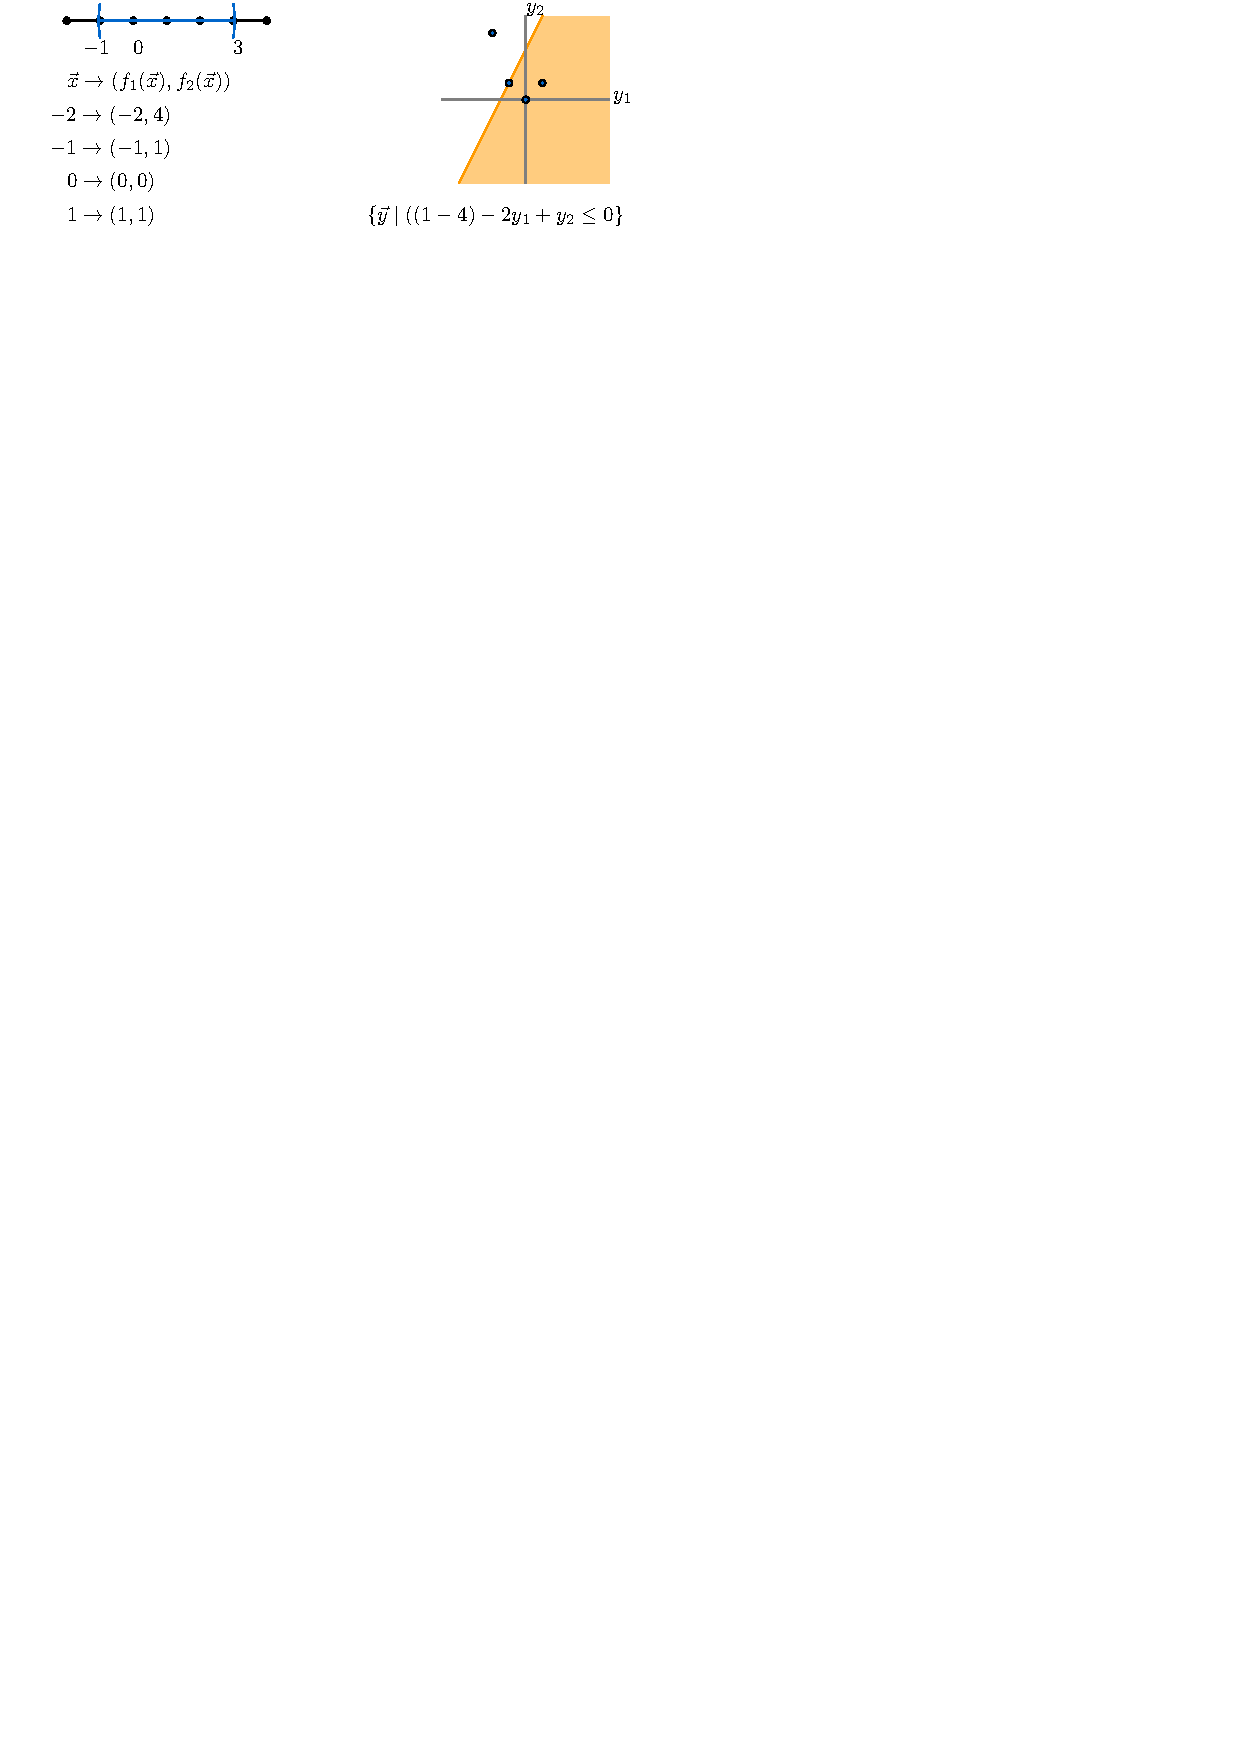
\includegraphics{../algebraic}
    \caption{algebra}
    \label{fig:algebraic}
\end{figure}

\section{Omitted Proofs}
\label{App:Omitted_Proofs}

\subsection{Proving Lemma~\ref{lemma:uncertain_intersection}}

In Section~\ref{sec:pointline} we describe a data structure solution for the visibility query between an entity $r$ that can move through edges of a simple polygon $P$ and a stationary entity $q$. Using ray shooting, we identify a polyline which consist of at most $n$ uncertain edges, where each uncertain edge has a corresponding reflex vertex. 
We are interested in computing if there is an uncertain edge $e$ together with a reflex vertex $v$, such that the line-of-sight of from $q$ through $v$, intersects the trajectory $r$ and we do this using semi-algebraic range searching. This proof is illustrated by Figure~\ref{fig:pointline}. In semi-algebraic range searching the object pair $(e,v)$ must be represented as a parameter vector $\vec{x}$. The most natural parameter vector would be a six-dimensional vector that specifies the start and end point of $e$, and the location of $v$. The trajectory of $r$ together with $q$ can be represented by a six-dimensional vector in the same way. However, earlier in this appendix we mentioned that a more efficient parametrization leads to a more efficient linearization. We use geometric observations that allow us to represent the edge $e$ and the trajectory $r$ by their full lines, thus reducing the number of variables needed.

\begin{figure}[h]
    \centering
    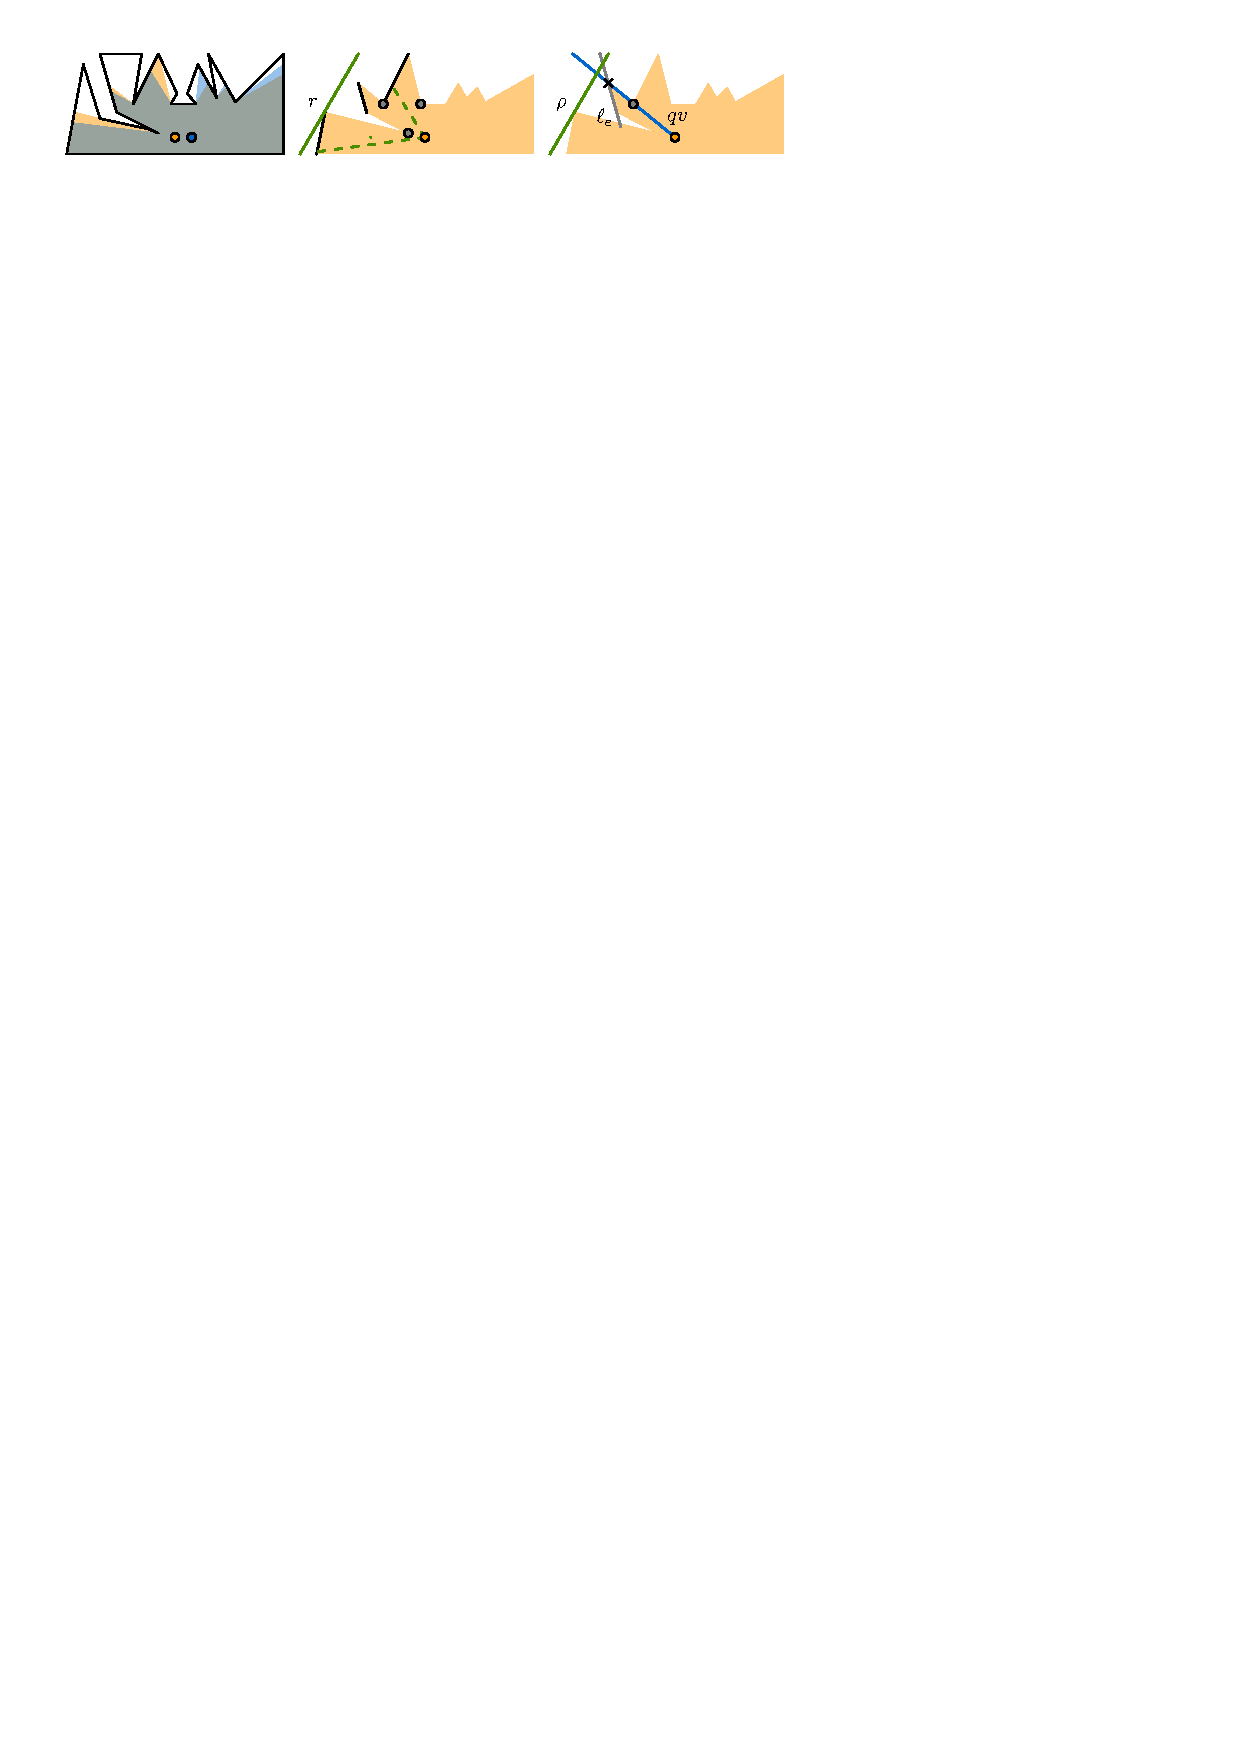
\includegraphics[]{../pointline}
    \caption{ (left) Two points in orange and blue, which have the same implicit visibility polygon, however there could be several placement of $r$ such that $r$ only intersects one of the two explicit visibility polygons. (middle) Entity $r$ in green, $q$ in orange and the chain of uncertain edges. (right) An illustration of the geometric argument. We compute the intersection between $\ell_e$ and $qv$ and check if that point lies below or above $\rho$.}
    \label{fig:pointline}
\end{figure}

\begin{proof}[Proof of Lemma~\ref{lemma:uncertain_intersection}]
For each uncertain edge $e \in U$ with corresponding reflex vertex $v$, we know that the line $qv$ intersects the line $\ell_e$ supporting $e$ on the domain of $e$ (this property is guaranteed by the construction of Aronov \etal). Recall that $\rho$ is the line that entity $r$ traverses. Per construction the entity $q$ lies below the line $\rho$, and the second level of our data structure guarantees that the intersection point between $qv$ and $\rho$ lies on the trajectory of $r$. It follows that $q$ can see $r$ if and only if, the intersection point $(x,y)$ between $qv$ and $\ell_e$ lies above $\rho$. Given $\rho, q, v$ and $\ell_e$, we can algebraically compute this intersection point $(x,y)$. We then substitute the equation for $(x, y)$ into the equation for $\rho$ and the point $(x,y)$ lies above this line if and only if the result is greater than $0$:

\[
vq := \left\{x,y \mid 0 =  \frac{x_4 - a_4}{x_3 - a_3} x - \frac{x_4 - a_4}{x_3 - a_3}x_3 + x_4  \right\}
\]

The lines $vq$ and $\ell_e$ intersect at the point where their $y$-coordinate is equal and therefore:


\begin{align*}
    x_1 x - x_2 =  \frac{x_4 - a_4}{x_3 - a_3} x - \frac{x_4 - a_4}{x_3 - a_3}x_3 + x_4 \\
    (x_3 - a_3)(x_1 x - x_2) = (x_4 - a_4) x - (x_4 - a_4)x_3 + (x_3 - a_3) x_4 \\
    (x_3 - a_3)x_1 x - (x_4 - a_4) x = x_2 (x_3 - a_3) - (x_4 - a_4)x_3 + (x_3 - a_3) x_4 
\end{align*}


From this equation we can extract the coordinates of the intersection point $(x,y)$ between $vq$ and $\ell_e$:

\begin{align*}
    x = \frac{x_2 (x_3 - a_3) - (x_4 - a_4)x_3 + (x_3 - a_3) x_4}{ (x_3 - a_3)x_1 - (x_4 - a_4)} \\
    y = x_1 \frac{x_2 (x_3 - a_3) - (x_4 - a_4)x_3 + (x_3 - a_3) x_4}{ (x_3 - a_3)x_1 - (x_4 - a_4)} - x_2
\end{align*}

Lastly we substitute the algebraic expression for $(x,y)$ into the formula for $\rho$ and we linearize the predicate:

\begin{align*}
    0 \ge a_1 (x_2 (x_3 - a_3) - (x_4 - a_4)x_3 + (x_3 - a_3) x_4) - \\
    x_2 - x_1 (x_2 (x_3 - a_3) - (x_4 - a_4)x_3 + (x_3 - a_3) x_4) + x_2 \\
    0 \ge [-a_1 a_3] (x_2) + [a_3]( x_1 x_2) + [a_1] (x_2 x_3) + [a_1a_4] (x_3) + \\
    [- a_4] (x_1 x_3) + [- a_1 a_3]( x_4) + [a_3] (x_1 x_4) + [-1](x_1 x_2 x_3)
\end{align*}

Thus we found a predicate $F(\vec{x}, \vec{a})$ with:

\begin{align*}
    (f_1, f_2, f_3, f_4, f_5, f_6, f_6, f_8) = (x_2, x_1x_2, x_2x_3, x_3, x_1x_3, x_4, x_1x_4, x_1x_2x_3) \\
    (g_0, g_1, g_2, g_3, g_4, g_5,g_6, g_7,g_8) = (0, -a_1a_3, a_3, a_1, a_1a_4, -a_4, -a_1a_3, a_3, -1)
\end{align*}

We can map every uncertain edge plus its reflex vertex to a point in $\mathbb{R}^8$ using the $f$-maps provided by the predicate. Any query consisting of the line $\rho$ and the point $q$ gets mapped to a halfspace in $\mathbb{R}^8$. The line $\rho$ (and with it, the trajectory of $r$) intersects an edge in $U$ if and only if its representative point lies in this halfspace. 
\end{proof}


\subsection{The proof of Lemma~\ref{lemma:hyperbola} }

In Section~\ref{sec:lineline} we study the line-of-sight between two entities that each move along a linear trajectory (possibly at different but constant speeds) during the time $t \in [0,1]$. Consider at all times $t \in [0,1]$ the line through the two entities, we can dualize this line to a point using classical point-line dualization. In Section~\ref{sec:lineline} we claim that the continuous dualization of the line through the two entities traces a degree-2 curve segment in the dual. Here we show why this is the case:

\begin{proof}[Proof of Lemma~\ref{lemma:hyperbola}]
Recall that we required that entity $q$ walks from $(a_1, a_2)$ to $(a_1 + a_3, a_2 + a_4)$ and that entity $r$ walks from $(a_5, a_6)$ to $(a_5 + a_7, a_6 + a_8)$. We can parametrize the position of entity $q$ and $r$ on the time $t$ as follows:

\begin{equation}
    \label{eq:line}
     q(t) = \left( \begin{array}{c}
         x_{q(t)}  \\
         y_{q(t)} 
    \end{array}  \right) = 
    \left( \begin{array}{c}
         a_1 + a_3 t \\
         a_2 + a_4 t
    \end{array}  \right)  \quad
      r(t) = \left( \begin{array}{c}
         x_{r(t)}  \\
         y_{r(t)} 
    \end{array}  \right) = 
    \left( \begin{array}{c}
         a_5 + a_7 t \\
         a_6 + a_8 t
    \end{array}  \right) 
\end{equation}


At all times, the line $\Gamma(t)$ represents the line through $q(t)$ and $r(t)$. We say that at all times, $\Gamma(t)$ has slope and offset $(\alpha(t), \beta(t))$. The parametrisation of $\Gamma(t)$ then becomes:

\begin{equation}
\label{eq:curve}
   \Gamma(t) = \left( \begin{array}{c}
         \alpha(t)  \\
         \beta(t) 
    \end{array}  \right) = 
    \left( \begin{array}{c}
         \frac{y_{r(t)} - y_{q(t)}}{x_{r(t)} - x_{q(t)}}  \\
         \alpha(t)\cdot x_{q(t)} - y_{q(t)}
    \end{array}  \right) =
    \left( \begin{array}{c}
         \frac{ a_6 - a_2 + (a_8 - a_4) t}
      { a_5 - a_1  + (a_7 - a_3) t }  \\
         \alpha(t) (a_1 - a_3 t) - a_2 - a_4 t 
    \end{array}  \right)
  \end{equation}
  
  If the time $t$ lies between $0$ and $1$, this parametric equation traces our curve segment $\gamma$ and if we take $t$ over all of $\mathbb{R}$, the parametric equation traces a full curve $\Gamma$. To show the degree of the curve $\Gamma$ we rewrite the parametrized curve to a canonical form that drops the dependence on $t$. First we take the formula for the $\beta$-coordinate and isolate $t$:
  
  \[
     t = \frac{\alpha(t) a_1 - a_2  - \beta(t)}{\alpha(t) a_3 + a_4}
  \]
We then take the formula for the $\alpha$-coordinate and remove the fraction by multiplying both sides with $ ((a_5 - a_1)  + (a_7 - a_3) t)$:

\[ 
\alpha(t)(a_5 - a_1)  + \alpha(t)(a_7 - a_3) t = (a_6 - a_2) + (a_8 - a_4) t
\]

We substitute the value for $t$ into this equation, and remove the fraction by multiplying both sides with $(\alpha(t) a_3 + a_4)$:

\begin{align*}
\alpha(t)(\alpha(t) a_3 + a_4)(a_5 - a_1)  + \alpha(t)(a_7 - a_3) (\alpha(t) a_1 - a_2  - \beta(t)) = \\
(a_6 - a_2)(\alpha(t) a_3 + a_4) + (a_8 - a_4) (\alpha(t) a_1 - a_2  - \beta(t)) \Rightarrow \\
\alpha(t)^2a_3(a_5 - a_1) + \alpha(t)a_4(a_5 - a_1)  + \alpha(t)^2a_1(a_7 - a_3)
- \alpha(t)a_2(a_7 - a_3)  - \alpha(t)\beta(t)(a_7 - a_3) = \\
\alpha(t) a_3(a_6 - a_2) + a_4(a_6 - a_2) + \alpha(t)a_1(a_8 - a_4) - a_2 (a_8 - a_4) - \beta(t)(a_8 - a_4) 
\end{align*}

Lastly we linearize this equation by separating polynomials based on $\alpha(t)$ and $\beta(t)$ from polynomials based on $a_1 \ldots a_8$.

\begin{align}
\label{eq:hyperbola}
    0= [\alpha(t)^2](a_5 a_3 -2 a_1 a_3 + a_1 a_7)+ \\
    [\alpha(t)](a_4 a_5 - a_3 a_6 + a_2 (2 a_3 - a_7) - a_1 a_8) + \\
    [\alpha(t)\beta(t)](-(a_7 - a_3)) + [\beta(t)](-(a_8 - a_4)) + [1](a_4(a_6 - a_2)- a_2 (a_8 - a_4))
\end{align}
\end{proof}

\subsection{The proof of Lemma~\ref{lemma:15000}}

In Section~\ref{sec:intersectionsearch} we describe how to preproces a convex simple polygon $P_E$ formed by a set of edges $E$ such that for any segment $\gamma$ of an arbitrary degree-2 curve $\Gamma$, we can test if $P_E$ is intersected by $\gamma$ in sub-linear time. In the section we explain that we first make many geometric observations about $P_E$ and that we only implore semi-algebraic range searching in the last step. We note that it is possible to immediately implore semi-algebraic range searching but that this leads to a less efficient solution. Although this solution brings worse bounds, the solution is more general: We specifically prove that we can preprocess \emph{any} set of edges $E$, such that we can test for an intersection between an arbitrary degree-2 curve segment $\gamma$ and an edge in $E$ in sub-linear time.  This means that the set of edges $E$ does not have to be connected, convex or even non-intersecting. We first provide a proof outline and then the formal proof.

\paragraph*{Proof outline of Lemma~\ref{lemma:15000}}
As an object set we are given a set $E$ of arbitrary edges with no restrictions. We say that an edge $e \in E$ goes from the point $(x_1, x_2)$ to the point $(x_1 + x_3, x_2 + x_4)$ and thus parametrize each edge as a vector $\vec{x} = (x_1, x_2, x_3, x_4)$. As a query family, we are given the family $\Gamma$ of degree-2 curve segments which are parametrized according to equation~\ref{eq:hyperbola} with a parametrization vector $\vec{a} = (a_1 \ldots a_8)$. The goal is to design a predicate function $F(\vec{x}, \vec{a})$ that takes any pair of edge and query curve and that outputs a number. The query curve should intersect the edge if and only if the output number is less than zero. Specifically, we design \emph{four} predicate functions $F_1, F_2, F_3, F_4$ and the query curve intersects the edge if and only if all four predicates output a number less than zero. This can be checked by using four consecutive halfspace-range queries.

We detect for an intersection between an arbitrary $\gamma$ in three steps:
\begin{enumerate}
    \item First we rotate and shear the plane, using the parameter vector $\vec{x}$, such that the edge $e$ starts at $(0,0)$ and ends at $(0, \lVert (x_3, x_4) \rVert$. We now know, that $\gamma$ can only intersect the edge at a point where its $x$-coordinate is $0$. 
    \item We algebraically compute the at most 2 times $t, t'$, where the $x$-coordinate of the full curve supporting $\gamma$ is zero and we check if $0 \le t, t' \le 1$. This gives the first two predicate functions $F_1, F_2$. If this is not the case for either $t$, then we know that $\gamma$ cannot intersect the edge $e$.
    \item As a third step, we fill in the times $t, t'$ where the first coordinate of the curve supporting $\gamma$ is zero and we check if the second coordinate lies between $0$ and $ \lVert (x_3, x_4) \rVert$. If this is not the case, then the curve goes over or under the line segment. This gives the last two predicate functions $F_3$ and $F_4$.
\end{enumerate}

Having computed the predicates $F_1, F_2, F_3, F_4$, we need to linearize them. And we linearize them using approximately 15000 terms. We want to briefly mention why this number is so high. In its general form, the predicate has twelve unrestricted variables $x_1 \ldots x_4$ and $a_1 \ldots a_8$. One can imagine, that twelve unrestricted variables leads to a formula with at least twelve linear terms.

At step 2, we compute the time $t$ for which the first coordinate of the degree-2 curve is zero. To do this, we need to make use of the quadratic equation and that will give us a square root containing both variables from $\vec{x}$ and $\vec{a}$. If we want to linearize, we need to get rid of the square root. That means squaring both sides and expanding the resulting equation which implies quadratically many more linear terms. At step 3, a similar thing happens and we again have to resolve a square root. We started with $12$ terms and we squared twice, which would naively give us $20.000$ terms.



\subsubsection{A proof of a more restricted case that linearizes to $\mathbb{R}^3$.}
We first want to show that the approach that we suggested above can be an efficient way to compute the intersection between algebraic objects. If you are only interested in the formal proof of Lemma~\ref{lemma:15000}, please skip ahead to the next subsection.

Consider the set $E$ of arbitrary line segments, and the family of regions $\Gamma'$ where each range $G \in \Gamma'$ is a \emph{line segment} (hence, a more restricted degree-2 curve). Agarwal notes \cite{agarwal1996range} that the intersection between an edge $e \in E$ and segment $G \in \Gamma$ can be written as a predicate with three linear terms. Most likely, Agarwal uses the cross product between the segments for this linearization and this approach does not generalize to curves. We show that with our approach, you also get a linearization of three terms. 

We assume that each edge $e$ in $E$ is from the point $(x_1, x_2)$ to $(x_1 + x_3, x_2 + x_4)$ and that each query $G$ in $\Gamma'$ is a segment from the point $(a_1, a_2)$ to $(a_1 + a_3, a_2 + a_4)$. The first step is to translate and shear the plane.
First we translate the plane with the vector $-(x_1, x_2)$ such that $e$ starts at the origin. Then we shear the plane with the following map: $(x,y) \rightarrow (x - \frac{x_3}{x_4}y, y)$ such that $e$ points upwards. 
If we apply our translation and shearing, we get a new segment $G'(t)$ whose parametrization on $t$ is:

\begin{align*}
    &G'(t) = R(x_3, x_4) \cdot (G(t) - (x_1, x_2)) =  
    \left( \begin{array}{c}
         x  \\
         y 
    \end{array} \right) =
    \left( \begin{array}{c}
         (a_1 - x_1 + t a_3) - \frac{x_3}{x_4}(a_2 - x_2 + t a_4 )  \\
         a_2 - x_2 + t a_4 
    \end{array} \right)
\end{align*}
The first thing that we do, is that we compute the time $t^*$ for which the $x$-coordinate of this transformed query segment $G'(t)$ is zero.

\begin{align*}
    x = 0 \Rightarrow \\
    0 = (a_1 - x_1 + t a_3) - \frac{x_3}{x_4}(a_2 - x_2 + t a_4 )   \Rightarrow \\
    - t ( a_3 -  \frac{x_3}{x_4} a_4) = a_1 - x_1 - \frac{x_3}{x_4} (a_2 - x_2) \Rightarrow \\
    %
    t = \frac{   a_1 - x_1 - \frac{x_3}{x_4} (a_2 - x_2)}{ - a_3 + \frac{x_3}{x_4}a_4}
\end{align*}

The first predicate verifies whether or not $t^*$ is greater or equal than $0$:

\begin{align*}
    0 \le t \Rightarrow \\
   0 \le F_1(\vec{x}, \vec{a}) = a_1 - x_1 - \frac{x_3}{x_4} (a_2 - x_2)  \\
    %
    0 = (a_1) + (1)[\frac{x_3}{x_4}x_2 - x_1] + (a_2) [ - \frac{x_3}{x_4} ] \\
    \textnormal{Hence we have a predicate } F_1 \textnormal{ Where }\\
    %
    A_0(\vec{a}) = a_1, \quad A_1(\vec{a}) = 1,\quad A_2(\vec{a}) = a_2 \\
    %
    f_1(\vec{x}) = \frac{x_3}{x_4}x_2 - x_1 \quad f_2(\vec{x}) = - \frac{x_3}{x_4}
\end{align*}

The second predicate verifies whether or not $t^*$ is lesser or equal to $1$:

\begin{align*}
    &t \le 1 \Rightarrow \\
    & a_1 - x_1 - \frac{x_3}{x_4} (a_2 - x_2) \le  - a_3 + \frac{x_3}{x_4}a_4 \\
    & a_1 - x_1 - \frac{x_3}{x_4} (a_2 - x_2) + a_3 - \frac{x_3}{x_4}a_4 \le 0 \\
    %
    &0 \ge F_2(\vec{x}, \vec{a}) = (a_1 + a_3) + (1)[\frac{x_3}{x_4}x_2- x_1] + (a_2 + a_4) [ - \frac{x_3}{x_4} ] \\
    %
    \textnormal{Hence we have a predicate } F_2 \textnormal{ Where } \\
    %
    &A_0(\vec{a}) = a_1 + a_3, \quad A_1(\vec{a}) = 1,\quad A_2(\vec{a}) = a_2 + a_4 \\
    %
    &f_1(\vec{x}) = \frac{x_3}{x_4}x_2- x_1,\quad f_2(\vec{x}) = - \frac{x_3}{x_4}
\end{align*}

The third predicate, verifies whether not the $y$ value of $G'(t^*)$ lies below $\sqrt{x_3^2 + x_4^2}$:

\begin{align*}
    y_{G'(t^*)} = a_2 - x_2 + t^* a_4   \le \sqrt{x_3^2 + x_4^2} \Rightarrow \\
    %
    a_2 - x_2 + a_4 \frac{   a_1 - x_1 - \frac{x_3}{x_4} (a_2 - x_2)}{ - a_3 + \frac{x_3}{x_4}a_4} \le \sqrt{x_3^2 + x_4^2} 
\end{align*}

We multiply both sides by $- a_3 + \frac{x_3}{x_4}a_4$ and obtain:


\begin{align*}
    (- a_2 a_3) +  (a_2 a_4) \left[\frac{x_3}{x_4}\right] +  (a_3)[x_2] + (a_4)[ - \frac{x_3}{x_4}x_2] + (a_4 a_1) + (a_4)[ \frac{x_3}{x_4}x_2 - x_1] - (a_2a_4)\left[\frac{x_3}{x_4}\right]
        \le \\
    (- a_3)[ \sqrt{x_3^2 + x_4^2} ] + (a_4) [\frac{x_3}{x_4} \sqrt{x_3^2 + x_4^2}] \Rightarrow \\
    (a_1 a_4 - a_2 a_3) + (a_3)[x_2 - \sqrt{x_3^2 + x_4^2}] + (a_4)[ - \frac{x_3}{x_4}( x_2 + \sqrt{x_3^2 + x_4^2}) -x_1 ] \le 0 \\
        %
    \textnormal{Hence we have a predicate } F_2 \textnormal{ Where } \\
    %
    A_0(\vec{a}) = a_1 a_4 - a_2 a_3, \quad A_1(\vec{a}) = a_3, \quad A_2(\vec{a}) = a_4 \\
    %
   f_1(\vec{x}) = \frac{x_3}{x_4}, \quad f_2(\vec{x}) =  x_2 - \sqrt{x_3^2 + x_4^2}, \quad f_3(\vec{x}) = - \frac{x_3}{x_4}( x_2 + \sqrt{x_3^2 + x_4^2}) -x_1
\end{align*}

The predicate $F_4$ checks if the $y$-value is above $0$. It is the same predicate as $F_3$ with the terms dependent on $\sqrt{x_3^2 + x_4^2}$. It follows that we can verify if a query segment intersects an edge in $E$ using four predicates which each have at most 3 terms. 

\subsubsection{The formal proof of Lemma~\ref{lemma:15000}}

Lastly, we provide the formal proof for Lemma~\ref{lema:15000}. Denote by $\gamma$ any segment parametrized by a vector $\vec{a}$ according to equation~\ref{eq:hyperbola}. The algebraic formulations will get very long, so for succinctness we denote $A_i = a_i - a_{i-4}$. The formulation for $\gamma$ dependent on $t$ now becomes:

\begin{equation}
  \gamma(t) = \left( \begin{array}{c}
         x  \\
         y 
    \end{array}  \right) =  
        \left( \begin{array}{c}
         \frac{ A_6 + A_8 t}
      { A_5  + A_7 t } \\
         a(t)(a_1 +  a_3 t) - a_2 -  a_4 t 
    \end{array}  \right)
\end{equation}

Removing brackets and applying the translation gives:

  \begin{equation*}
   \gamma(t)_T = \left( \begin{array}{c}
         x  \\
         y 
    \end{array}  \right) = 
    \left( \begin{array}{c}
         \frac{ A_6 + A_8 t}
      { A_5  + A_7 t } - x_1 \\
         \frac{ A_6 a_1 + A_8 a_1 t + A_6 a_3 t + A_8 a_3 t^2 }{A_5 + A_7t} - a_2 - a_4 t - x_2
    \end{array}  \right)
  \end{equation*}
  
We then apply the shearing and obtain $\gamma(t)'$ just as in the previous subsection:

\begin{equation*}
   \overline{\gamma(t)'} = \left( \begin{array}{c}
         x  \\
         y 
    \end{array}  \right) = 
    \left( \begin{array}{c}
       \frac{ A_6 + A_8 t}
      { A_5  + A_7 t } - x_1 - \frac{x_3}{x_4} \left( \frac{ A_6 a_1 + A_8 a_1 t + A_6 a_3 t + A_8 a_3 t^2 }{A_5 + A_7t} - a_2 - a_4 t - x_2 \right)  \\
      %
         \frac{ A_6 a_1 + A_8 a_1 t + A_6 a_3 t + A_8 a_3 t^2 }{A_5 + A_7t} - a_2 - a_4 t - x_2
    \end{array}  \right)
\end{equation*}

\paragraph*{Verifying that $0 \le t^* \le 1$}

The first thing that we do, is verify the time $t^*$ for which $x=0$. We check if this value lies below 1 and this gives our first predicate $F_1$. The formulation for $F_2$ follows from $F_1$. Below we equate $x$ to $1$ and  multipy each side of the equality with $(A_5 + A_7 t)$. Then we apply the quadratic equation to find the time(s) $t^*$ for which the $x$-coordinate is zero.

\begin{align*}
     A_6 + A_8 t - (x_1 + a_2 + x_2 + a_4t)(A_5 + A_7 t) - \frac{x_3}{x_4} (A_6 a_1 + A_8 a_1 t + A_6 a_3 t + A_8 a_3 t^2) = 0  \Rightarrow \\
     \textnormal{Quadratic equation:} \\
     [t^2](- a_4 A_7 - a_3 A_8 \frac{x_3}{x_4}) + \\
     [t] (- a_4A_5 - a_2A_7+ A_8- A_7 x_1 - A_7 x_2 - (a_3A_6 + a_1 A_8)\frac{x_3}{x_4}) + \\
     [1] (a_2 A_5 + A_6- A_5x_1  - A_5x_2  - a_1A_6 \frac{x_3}{x_4})
\end{align*}

We want to demand that $t^* \le 1$. We first do this using just the variables $a,b,c$ from the quadratic equation:

\begin{align*}
     1 \ge quadratic-equation \Rightarrow \\
    2c \ge -b + \sqrt{b^2 - 4 ac} \Rightarrow \\
    4c^2 + 4bc + b^2 \ge b^2 - 4 ac \Rightarrow \\
    (c^2 - bc + ac) \ge 0 
\end{align*}


Now we work out what the terms in this equation actually are: 

\paragraph*{Working out $c^2$:}

\begin{align*}
    c^2 = \left(a_2 A_5 + A_6- A_5x_1  - A_5x_2  - a_1A_6 \frac{x_3}{x_4} \right)^2 = \\
    \left[\frac{x_3}{x_4}(x_1 + x_2)\right]( 2 a_1 A_6 A_5) + 
    [x_1 + x_2](- 2 a_2 A_5^2 - 2 A_6 A_5) +\\
    [x_1^2 + x_2^2](A_5^2) +
    [x_1x_2](2A_5^2) +
   \left [\left( \frac{x_3}{x_4} \right)^2 \right](a_1^2 A_6^2) + \\
    \left[\frac{x_3}{x_4}\right]( - 2 a_1 a_2 A_6 A_5  - 2 a_1 A_6^2) +
    [1](a_2^2 A_5^2+ 2 a_2 A_6 A_5+ A_6^2)
\end{align*}


\paragraph*{Working out the $ac$:}

\begin{align*}
    ac = 
     \left[\frac{x_3}{x_4}(x_1 + x_2)\right](a_3 A_5 A_8) + \\
     [x_1 + x_2](a_4 A_5 A_7) +\\
    \left [\left( \frac{x_3}{x_4} \right)^2 \right](a_1 a_3 A_6 A_8) +\\
      \left[\frac{x_3}{x_4}\right](a_1 a_4 A_6 A_7- a_2 a_3 A_5 A_8- a_3 A_6 A_8) +\\
     [1](- a_2 a_4 A_5 A_7 - a_4 A_6 A_7)
\end{align*}

\paragraph{Working out the $bc$:}

\begin{align*}
     bc =
     \left[\frac{x_3}{x_4}(x_1 + x_2)\right](a_1 A_6 A_7 + a_1 A_5 A_8 + a_3 A_5 A_6) + \\
     [x_1 + x_2](  a_4 A_5^2- A_6 A_7- A_5 A_8) +\\
    [x_1^2 + x_2^2](A_5 A_7) + \\
    [x_1x_2](2 A_5 A_7) \\
    \left [\left( \frac{x_3}{x_4} \right)^2 \right](a_1^2 A_6 A_8+ a_3 a_1 A_6^2 ) + \\
    \left[\frac{x_3}{x_4}\right](  a_4 a_1 A_5 A_6+ a_2 a_1 A_6 A_7- a_2 a_1 A_5 A_8- 2 a_1 A_6 A_8- a_3 A_6^2- a_2 a_3 A_5 A_6) +\\  [1](A_6 A_8- a_2 a_4 A_5^2- a_4 A_5 A_6 - a_2^2 A_5 A_7 - a_2 A_6 A_7 + a_2 A_5 A_8)
\end{align*}


Concatenating these results gives the predicate $F_1$. The predicate $F_2$ is simpler than $F_1$. In our formulation of $c^2, ac, bc$ we already separated terms based on $\vec{x}$ and terms based on $\vec{a}$ and surprisingly, we end up with only 10 non-separable terms. This means that we can check predicate $F_1$ and $F_2$ with a halfspace-emptyness query in $\mathbb{R}^10$ which is not so bad. However, from this point on it is going to get worse:
From the quadratic equation we know that $t^* = \frac{-b \pm \sqrt{b^2 - 4ac}}{2c}$ and with the previous predicates, we can determine if $t^*$ lies within the relevant interval. The next step is to check if at time $t^*$, the $y$-value of the hyperbola is between $0$ and $C =\sqrt{x_3^2 + x_4^2}$.




\begin{align*}
     y_{\gamma(t)'} \le C \Rightarrow \\
\frac{ A_6 a_1 + A_8 a_1 t + A_6 a_3 t + A_8 a_3 t^2 }{A_5 + A_7t} - a_2 - a_4 t - x_2 \le C \Rightarrow \\
%
      \textnormal{Grouping variables on t} \\
[t^2](A_8 a_3-a_4 A_7) + \\
[t](A_8 a_1+ A_6 a_3 - a_4 A_5- a_2 A_7 - A_7x_2 - A_7 C) + \\
[1](A_6 a_1- a_2 A_5 - A_5 x_2 - A_5 C)   \le 0 \\
%
\end{align*}

At this point, we substitute the result of the quadratic equation into $t$. After this substitution we will have the term $\sqrt{D} = \sqrt{b^2 - 4ac}$ whose variables depend on both $\vec{x}$ and $\vec{a}$. To linearize this function, we have to take $\sqrt{D}$ apart and square both sides. We substitute the value for $t$ with the result of the quadratic equation and multiply both sides with $4c^2$:

\begin{align*}
[ b^2 - 2b\sqrt{D} + D](A_8 a_3-a_4 A_7) + \\
[-2bc -2c\sqrt{D})](A_8 a_1+ A_6 a_3 - a_4 A_5- a_2 A_7 - A_7x_2 - A_7 C) + \\
[4c^2](A_6 a_1- a_2 A_5 - A_5 x_2 - A_5 C) \le 0 \\
\end{align*}

Consider the equation $(b^2 + c^2 - bc + ac)$. At this point, a conservative estimate for the number of non-separable terms based on $\vec{a}$ and $\vec{a}$ in this equation would be $12$ terms. These expressions are multiplied with at least $7$ non-separable terms. Now we take $\sqrt{D}$ to one side (and with it, several polynomials based on both $\vec{x}$ and $\vec{a}$) and we square both sides. This will lead to around $(12\cdot 7)^2 * 2$ non-separable terms. Approaching the $15000$ non-separable terms. We ran this computation using algebraic-simplification software and it seems like you cannot group expressions to reduce the total number of terms.



\end{document}
